\documentclass[11pt]{article}

% 
\usepackage{natbib}
%\bibliographystyle{unsrtnat}
\bibliographystyle{unsrt}

% change document font family to Palatino, and code font to Courier
\usepackage{mathpazo} % add possibly `sc` and `osf` options
\usepackage{eulervm}
\usepackage{courier}
%allow formula formatting
\usepackage{amsmath}
\DeclareMathAlphabet\mathbfcal{OMS}{cmsy}{b}{n}
\usepackage{comment}
\usepackage{enumerate}
\usepackage{xcolor}
\usepackage{algorithm}
\usepackage{algpseudocode}
%title positon
\usepackage{titling} %fix title
\setlength{\droptitle}{-6em}   % Move up the title 

\usepackage{verbatim}
% change page margin
\usepackage[margin=1 in]{geometry} 
\usepackage{subfigure}
%allow inserting multiple graphs
\usepackage{subfig}
\usepackage{graphicx}
\usepackage{float}
%allow code chunks
\usepackage{listings}
\lstset{basicstyle=\footnotesize\ttfamily,breaklines=true}
\lstset{frame=lrbt,xleftmargin=\fboxsep, xrightmargin=-\fboxsep}

%declare sum int sign
\DeclareMathOperator*{\SumInt}{%
\mathchoice%
  {\ooalign{$\displaystyle\sum$\cr\hidewidth$\displaystyle\int$\hidewidth\cr}}
  {\ooalign{\raisebox{.14\height}{\scalebox{.7}{$\textstyle\sum$}}\cr\hidewidth$\textstyle\int$\hidewidth\cr}}
  {\ooalign{\raisebox{.2\height}{\scalebox{.6}{$\scriptstyle\sum$}}\cr$\scriptstyle\int$\cr}}
  {\ooalign{\raisebox{.2\height}{\scalebox{.6}{$\scriptstyle\sum$}}\cr$\scriptstyle\int$\cr}}
}

\usepackage{"./macro/GrandMacros"}
\usepackage{"./macro/Macro_BIO235"}
\begin{document}
\setlength{\parindent}{0pt}
%\setcounter{equation}{0}
%\renewcommand{\theequation}{1.1.\arabic{equation}}
%\paragraph{AIC and small sample correction}\mbox{}\\
%\label{1}  \eqref{1} 
%%%%%%%%%%%%%%%%%%%%%%%%%%%%%%%%%%%%%%%%%%%%%
%%%%%%%%%%%% TItle page with contents %%%%%%%%%%%%%%%
%%%%%%%%%%%%%%%%%%%%%%%%%%%%%%%%%%%%%%%%%%%%%

\title{CVEK-boot Report\\Wenying Deng \vspace{-1ex}}

\pretitle{\begin{flushright}\normalsize}
\posttitle{\par\end{flushright}}
\author{}
\date{}
\vspace{-10em}
\maketitle
\vspace{6em}


\tableofcontents
%%%%%%%%%%%%%%%%%%%%%%%%%%%%%%%%%%%%%%%%%%%%%
%%%%%%%%%%%% Formal Sections %%%%% %%%%%%%%%%%%%%%
%%%%%%%%%%%%%%%%%%%%%%%%%%%%%%%%%%%%%%%%%%%%%
\clearpage
\vspace{2em}
\section{{\bf Introduction}}
In recent years, kernel machine-based hypothesis tests (e.g. SKAT) for high-dimensional, nonlinear effects has seen widespread application in GWAS and gene-environment interaction studies. However, constructing a test for the interaction between groups of continuous features (for example, interaction between groups of air pollutants and multicategory nutrition intake) remains difficult in practice. The main challenges root from (1) constructing an appropriate main-effect kernel that induce unbiased estimator for the null model, and (2) constructing an appropriate interaction-effect kernel describing only the effect of between-groups interaction, which is necessary for building a valid test statistic. Recently, \citep{liu_robust_2017} addressed the first challenge by proposing cross-validated ensemble of kernels (CVEK), an ensemble-based estimator that adaptively learn the form of the main-effect kernel from data, and constructed an companion variance component test. While interesting, the null distribution of CVEK is constructed using asymptotic approximation, and requires the interaction-kernel to be fixed a priori, therefore calling into question the validity of the test in limited sample, and prevents practitioners from deploying flexible methods to learn the interaction kernel from data. In this work, we seek to address these shortcomings by proposing a bootstrap test for CVEK. We conduct comprehensive simulation study to evaluate the validity (i.e. Type I error) and power of the proposed test using diverse choices of modeling strategy and under a wide range of data-generation mechanisms. Our simulation results revealed valuable insight on the impact of choice of estimation strategy (i.e. choices of tuning-parameter selection criteria and ensemble strategy) on the performance of the resulting hypothesis test.

\newpage
\section{{\bf Method}}
\subsection{\textbf{Cross-validated Ensemble of Kernerls}}
\setcounter{equation}{0}
\renewcommand{\theequation}{2.1.\arabic{equation}}
\subsubsection{{Overview}}
Cross-validated Ensemble of Kernerls (CVEK) \citep{liu_robust_2017} is a ensemble-based method for an unknown data-generating function $h: \mathbb{R}^p\rightarrow \mathbb{R}$. Traditional practices for estimating $h$, for example  Gaussian Process (GP) regression using a single kernel function, tend to impose \textit{a priori} assumption on the mathematical property of $h$ by specifying the reproducing kernel function $k$ for $h \in \Hsc$, thereby risking inducing biased estimation and incorrect inference. To circumvent this issue, CVEK propose   estimating $h$ using the ensemble of GP predictions generated from a library of (fixed) base kernel functions $\{k_d\}_{d=1}^D$:
\begin{align}
\hat{h}(\bx)=\sum_{d=1}^D u_d\hat{h}_d(\bx), \quad \bu \in \Delta=\{\bu | \bu \geq 0, \parallel \bu \parallel_1=1\}
\end{align}
where $\hat{h}_d$ is the kernel predictor generated by $d^{th}$ base kernel $k_d$.\\
To be more specific, for each given basis kernel $\{k_d\}_{d=1}^D$, CVEK first estimate $\hat{\bh}_d=\bK_d(\bK_d+\hat{\lambda}_d\bI)^{-1}\by$, the prediction based on $d^{th}$ kernel, where the tuning parameter $\hat{\lambda}_d$ is selected by minimizing certain criteria (see section 1.2). After which, CVEK combines the the individual base kernel predictors $\{\hat{h}_d\}_{d=1}^D$ according to some ensemble strategy (see section 1.3). In addition to producing ensemble prediction $\hat{h}$, CVEK also produces an ensemble kernel matrix $\hat{\bK}$ which describes the mathematical property of the ensemble RKHS. $\hat{\bK}$ is estimated by solving:
\begin{align*}
\hat{\bK}(\hat{\bK}+\lambda \bI)^{-1}=\hat{\bA}
\end{align*}
In fact, $\hat{\bK}$ can be computed in closed form. If we denote $\bU_A$ and $\{\delta_{A,k}\}_{k=1}^n$ the eigenvector and eigenvalues of $\hat{\bA}$, then:
\begin{align*}
\hat{\bK}=\bU_A diag(\frac{\delta_{A,k}}{1-\delta_{A,k}})\bU_A^T
\end{align*}
A complete summary of the proposed procedure (using LooCV for tuning-parameter selection and empirical risk minimization for ensemble strategy) is available in Algorithm 1.


\subsubsection{{Tuning Parameter Selection}}
Models may provide a good fit to the training data, but it will not fit sufficiently well to the test data. Tuning parameter could be chosen to address this problem. Here we define four objective functions in terms of tuning parameter $\lambda \in \Lambda$ to be minimized. Denote
\begin{align}
\bA_\lambda=\bK(\bX, \bX)[\bK(\bX, \bX)+\lambda \bI]^{-1}
\end{align}
In this way, $tr(\bA_\lambda)$ is the effective number of model parameters, excluding $\mu$ and $\sigma^2$. It decreases monotonically with $\lambda>0$. Additionally, we denote $\by^\star$ as the centered $\by$: $\by^\star=\by-\hat{\bmu}$, where $\hat{\mu}=\frac{1}{n}\sum_{i=1}^ny_i$.

\paragraph{K-Fold and leave-one-out Cross Validation}\mbox{}\\
Cross validation is probably the simplest and most widely used method for estimating prediction error. Suppose we do a $K$-fold cross-validation, which partitions observations into $K$ groups, $\kappa(1),...,\kappa(K)$, and calculates $\bA_\lambda$ $K$ times, each time leaving out group $\kappa(i)$, to get $\bA_\lambda^{-\kappa(1)}, \bA_\lambda^{-\kappa(2)}$, etc. For $\bA_\lambda^{-\kappa(i)}$, cross-validated residuals are calculated on the observations in $\kappa(i)$, which did not contribute to estimating $\bA$. The objective function estimated prediction error and is the sum of the squared cross-validated residuals:
\begin{align}
\lambda_{K-CV}=\underset{\lambda \in \Lambda}{argmin}\;\Big\{log\sum_{i=1}^K[\by_{\kappa(i)}^\star-\bA_\lambda^{-\kappa(i)}\by_{\kappa(i)}^\star]^T[\by_{\kappa(i)}^\star-\bA_\lambda^{-\kappa(i)}\by_{\kappa(i)}^\star]\Big\}
\end{align}
LooCV is the situation when $K=n$. In this case, we can write our objective function as \citep{golub_generalized_1979}:
\begin{align}
\lambda_{n-CV}=\underset{\lambda \in \Delta}{argmin}\;\Big\{log\;\by^{\star T}[\bI-diag(\bA_\lambda)-\frac{1}{n}\bI]^{-1}(\bI-\bA_\lambda)^2[\bI-diag(\bA_\lambda)-\frac{1}{n}\bI]^{-1}\by^\star \Big\} \label{3}
\end{align}

The value $K$ influences bias and variance of cross-validation. With $K=n$, the cross-validation estimator is approximately unbiased for the true (expected) prediction error because it almost use all the data in each training set. Therefore, it can have high variance because $n$ training sets are so similar to one another. Additionally, the computational burden is also considerable, requiring $n$ applications of the learning method. On the other hand, with larger $K$ such as 5 \citep{hastie_elements_2009} or 10, cross-validation will have lower variance, but making bias a problem.

\paragraph{Akaike Information Criteria}\mbox{}\\
Based on the idea of "model fit + model complexity", Akaike's Information Criterion (AIC) \citep{akaike_information_1998} chooses $\lambda$ by minimizing,
\begin{align*}
AIC=&2(p+2)-2log(\hat{L})\\
=&2(p+2)-2[-\frac{n}{2}log (\hat{\sigma}^2)-\frac{n}{2}log (2\pi)-\frac{1}{2\hat{\sigma}^2}\by^{\star T}(\bI-\bA_\lambda)^2\by^\star]\\
=&2(p+2)+n log[\frac{1}{n}\by^{\star T}(\bI-\bA_\lambda)^2\by^\star]+n+n log(2\pi)
\end{align*}
Drop the constant $n$ and divide it by $n$, we obtain our objective function:
\begin{align}
\lambda_{AIC}=\underset{\lambda \in \Lambda}{argmin}\Big\{log\; \by^{\star T}(\bI-\bA_\lambda)^2\by^\star+\frac{2[tr(\bA_\lambda)+2]}{n}\Big\} \label{1}
\end{align}
When $n$ is small, extreme overfitting is possible, giving small bias/ large variance estimates. The small-sample correction of AIC \citep{hurvich_regression_1989, hurvich_clifford_m._smoothing_2002} is derived by minimizing minus 2 times expected log likelihood, where we plug in $\bA_\lambda$ and $\hat{\sigma}^2$. In this case, we obtain our small-sample size objective function AICc:
\begin{align}
\lambda_{AICc}=\underset{\lambda \in \Lambda}{argmin}\Big\{log\; \by^{\star T}(\bI-\bA_\lambda)^2\by^\star+\frac{2[tr(\bA_\lambda)+2]}{n-tr(\bA_\lambda)-3}\Big\} \label{2}
\end{align}
Compare \eqref{1}  and \eqref{2} , it is easy to tell that AICc considers more of the model complexity since $\frac{n}{n-tr(\bA_\lambda)-3}>1$. It makes sense intuitively because it need to shrink more to prevent small bias/ large variance estimates.

\paragraph{Generalized Cross Validation}\mbox{}\\
In \eqref{3}, if we approximate each $A_{\lambda[ii]}$ with their mean $\frac{tr(\bA_\lambda)}{n}$, in a sense that we give equal weight to all observations. We get the Generalized Cross Validation (GCV) objective function:
\begin{align}
\lambda_{GCV}=\underset{\lambda \in \Lambda}{argmin}\Big\{log\; \by^{\star T}(\bI-\bA_\lambda)^2\by^\star-2log[1-\frac{tr(\bA_\lambda)}{n}-\frac{1}{n}]\Big\} \label{4}
\end{align}
The "$-\frac{1}{n}$" terms in \eqref{4} is because GCV counts $\mu$ as part of model complexity, but not $\sigma^2$. This motivates the proposed small-sample correction to GCV \citep{boonstra_small-sample_2015}, which does count $\sigma^2$ as a parameter:
\begin{align}
\lambda_{GCVc}=\underset{\lambda \in \Lambda}{argmin}\Big\{log\; \by^{\star T}(\bI-\bA_\lambda)^2\by^\star-2log[1-\frac{tr(\bA_\lambda)}{n}-\frac{2}{n}]_+\Big\}
\end{align}
Under this situation, perfect fit of the observations to the predictions, given by $\lambda=0$, cannot occur.


\paragraph{Generalized Maximum Profile Marginal Likelihood}\mbox{}\\
Suppose we relate $Y$ and $\bX$ by a linear model, $Y=\mu+\phi(\bX)^T\bbeta+\epsilon$, with $\epsilon \sim N(0, \sigma^2)$, where $\phi(\bx)$ is a function mapping a $D$-dimensional input vector $\bx$ into an $p$-dimensional feature space. If we assume $\bbeta$ are jointly and independently normal with mean zero and variance $\sigma^2/\lambda$, the penalty term matches the negative normal log-density, up to a normalizing constant not depending on $\bbeta$:
\begin{align*}
p_\lambda(\bbeta, \sigma^2)=\frac{\lambda}{2\sigma^2}\bbeta^T\bbeta-\frac{p}{2}log(\lambda)+\frac{p}{2}log(\sigma^2)
\end{align*}
One can consider a marginal likelihood, where $\lambda$ is interpreted as the variance component of a mixed-effects model:
\begin{align*}
m(\lambda, \sigma^2)=&log \int_{\bbeta} exp\{ l(\bbeta, \sigma^2)-p_\lambda(\bbeta, \sigma^2)\}d\bbeta \\=&-\frac{1}{2\sigma^2}\by^{\star T}(\bI-\bA_\lambda)\by^\star-\frac{n}{2}log(\sigma^2)+\frac{1}{2}log \mid \bI-\bA_\lambda \mid
\end{align*}
From this, $\by^\star |\lambda, \sigma^2$ is multivariate normal with mean $\mathbf{0}_n$ and covariance $\sigma^2(\bI-\bA_\lambda)^{-1}$. The maximum profile marginal likelihood (MPML) estimate, originally proposed for smoothing spline \citep{wecker_signal_1983}, profiles $m(\lambda, \sigma^2)$ over $\sigma^2$, replacing each instance with $\hat{\sigma}_\lambda^2=\by^{\star T}(\bI-\bA_\lambda)\by^\star/n$, and maximized the "concentrated" log-likelihood, $m(\lambda, \hat{\sigma}_\lambda^2)$:
\begin{align*}
\lambda_{MPML}=\underset{\lambda \in \Lambda}{argmin}\Big\{log\; \by^{\star T}(\bI-\bA_\lambda)\by^\star-\frac{1}{n}log \mid \bI-\bA_\lambda \mid \Big\}
\end{align*}
Closely related is the generalized/ restricted MPML \citep{harville_maximum_1977, wahba_comparison_1985}, which adjusts the penalty to account for estimation of regression parameter $\beta_0$ that is not marginalized, resulting in one degree of freedom:
\begin{align}
\lambda_{GMPML}=\underset{\lambda \in \Lambda}{argmin}\Big\{log\; \by^{\star T}(\bI-\bA_\lambda)\by^\star-\frac{1}{n-1}log \mid \bI-\bA_\lambda \mid \Big\} \label{5}
\end{align}


\paragraph{Relation between AIC, GCV and GMPML}\mbox{}\\
It's interesting to compare the $\lambda$'s selected from AIC, GCV, or GMPML, since AIC comes from Kullback-Leibler divergence, GCV from cross-validation and GMPML from likelihood. To do this, first we need to introduce some notations.\\
If we denote $\bU_K$ and $\{\eta_{K, j}\}_{j=1}^n$ the eigenvector and eigenvalues of $\bK$, then $\bA_\lambda$ adopts the form:
\begin{align*}
\bA_\lambda=\bU_K diag(\frac{\eta_{K, j}}{\eta_{K, j}+\lambda})\bU_K^T=\bU_K \bD_{K,\lambda}\bU_K^T
\end{align*}

\begin{comment}
As we can see from the two objective functions, $\lambda_{GCV}$ and $\lambda_{GMPML}$ share the same "model fit" term $log\; \by^{\star T}(\bI-\bA_\lambda)\by^\star$. Their difference focuses on "model complexity" terms, which is maximizing $2log[1-\frac{tr(\bA_\lambda)}{n}-\frac{1}{n}]$ for $\lambda_{GCV}$ and $\frac{1}{n-1}log \mid \bI-\bA_\lambda \mid$ for $\lambda_{GMPML}$. Up to a constant not depending on $\lambda$, the difference boils down to,
\begin{align}
&GCV: \; log[tr(\bI-\bA_\lambda)]=log[\sum_{j=1}^n\frac{\lambda}{\eta_{K, j}+\lambda}]\\
&GMPML: \; log\mid \bI-\bA_\lambda\mid=log[\prod_{j=1}^n\frac{\lambda}{\eta_{K, j}+\lambda}]
\end{align}

Take derivative of these two equations with respect to $\lambda$,
\begin{align*}
\frac{\partial }{\partial \lambda}log[tr(\bI-\bA_\lambda)]&=\frac{\sum_{j=1}^n\frac{\eta_{K, j}}{(\eta_{K, j}+\lambda)^2}}{\sum_{j=1}^n\frac{\lambda}{\eta_{K, j}+\lambda}}\\
\frac{\partial }{\partial \lambda}log\mid \bI-\bA_\lambda\mid&=\sum_{j=1}^n\frac{\eta_{K, j}}{\lambda(\eta_{K, j}+\lambda)}
\end{align*}
\end{comment}

Denote the objective functions in \eqref{1}, \eqref{4} and \eqref{5} as $f_{AIC}$, $f_{GCV}$ and $f_{GMPML}$, and calculate the derivatives of them with respect to $\lambda$ respectively,
\begin{align}
\frac{\partial f_{AIC}}{\partial \lambda}&=\frac{2tr\Big[\bU_K^T\by^\star \by^{\star T}\bU_K(\bD_{K, \lambda}-1)\frac{\partial \bD_{K, \lambda}}{\partial \lambda}\Big]}{tr[\bU_K^T\by^\star \by^{\star T}\bU_K(\bI-\bD_{K, \lambda})^2]}+\frac{2tr\Big(\frac{\partial \bD_{K, \lambda}}{\partial \lambda}\Big)}{n} \label{6} \\
\frac{\partial f_{GCV}}{\partial \lambda}&=\frac{2tr\Big[\bU_K^T\by^\star \by^{\star T}\bU_K(\bD_{K, \lambda}-1)\frac{\partial \bD_{K, \lambda}}{\partial \lambda}\Big]}{tr[\bU_K^T\by^\star \by^{\star T}\bU_K(\bI-\bD_{K, \lambda})^2]}+\frac{2tr\Big(\frac{\partial \bD_{K, \lambda}}{\partial \lambda}\Big)}{n-tr(\bA_\lambda)-1}  \label{7}\\
%\end{align}
%\begin{align}
\frac{\partial f_{GMPML}}{\partial \lambda}&=\frac{-tr\Big[\bU_K^T\by^\star \by^{\star T}\bU_K \frac{\partial \bD_{K, \lambda}}{\partial \lambda}\Big]}{tr[\bU_K^T\by^\star \by^{\star T}\bU_K(\bI-\bD_{K, \lambda})]}+\frac{tr\Big[(\bI-\bD_{K, \lambda})^{-1}\frac{\partial \bD_{K, \lambda}}{\partial \lambda}\Big]}{n-1}
\end{align}

Notice for $j^{th}$ element of diagonal vector of $\bD_{K, \lambda}$, its derivative with respect to $\lambda$ is negative,
\begin{align*}
\frac{\partial }{\partial \lambda}\Big[\frac{\eta_{K, j}}{\eta_{K, j}+\lambda}\Big]=-\frac{\eta_{K, j}}{(\eta_{K, j}+\lambda)^2}<0, \quad for\; j=1,\;2,...,\;n
\end{align*}
Further notice that the difference between \eqref{6} and \eqref{7} focuses on the second terms, both of which are increasing function of $\lambda$.
\begin{align*}
\frac{2tr\Big(\frac{\partial \bD_{K, \lambda}}{\partial \lambda}\Big)}{n-tr(\bA_\lambda)-1}<\frac{2tr\Big(\frac{\partial \bD_{K, \lambda}}{\partial \lambda}\Big)}{n}
\end{align*}
Therefore, when $\frac{\partial f_{AIC}}{\partial \lambda}=0$, $\frac{\partial f_{GCV}}{\partial \lambda}<0$, which means $\lambda_{AIC}<\lambda_{GCV}$.\\

\begin{comment}
On the other hand, we compare (2.1.12) and (2.1.13), and notice that,
\begin{align*}
\frac{-tr\Big[\bU_K^T\by^\star \by^{\star T}\bU_K\frac{\partial \bD_{K, \lambda}}{\partial \lambda}\Big]}{tr[\bU_K^T\by^\star \by^{\star T}\bU_K(\bI-\bD_{K, \lambda})^2]}>\frac{-tr\Big[\bU_K^T\by^\star \by^{\star T}\bU_K \frac{\partial \bD_{K, \lambda}}{\partial \lambda}\Big]}{tr[\bU_K^T\by^\star \by^{\star T}\bU_K(\bI-\bD_{K, \lambda})]}, \quad \frac{2tr\Big[\bU_K^T\by^\star \by^{\star T}\bU_K\bD_{K, \lambda}\frac{\partial \bD_{K, \lambda}}{\partial \lambda}\Big]}{tr[\bU_K^T\by^\star \by^{\star T}\bU_K(\bI-\bD_{K, \lambda})^2]}<0
\end{align*}

and if most of $\eta_{K, j}'s>\lambda$, then,
\begin{align*}
\frac{2tr\Big(\frac{\partial \bD_{K, \lambda}}{\partial \lambda}\Big)}{n}<\frac{tr\Big[(\bI-\bD_{K, \lambda})^{-1}\frac{\partial \bD_{K, \lambda}}{\partial \lambda}\Big]}{n-1}
\end{align*}

In this case, we obtain $\frac{\partial f_{AIC}}{\partial \lambda}<\frac{\partial f_{GMPML}}{\partial \lambda}$, which means $\lambda_{GMPML}<\lambda_{AIC}$.
\end{comment}

\begin{comment}
In terms of GCV and GMPML, probably we need the relative size of $\eta_{K, j}$'s and $\lambda$ to make a deterministic conclusion. To be more specific, we need to prove,
\begin{align*}
\frac{\partial }{\partial \lambda}\Big[log\; \by^{\star T}(\bI-\bA_\lambda)^2\by^\star\Big]>\frac{\partial }{\partial \lambda}\Big[log\; \by^{\star T}(\bI-\bA_\lambda)\by^\star\Big]
\end{align*}
And then, up to a constant not depending on $\lambda$, the difference boils down to,
\begin{align}
&GCV: \; log[tr(\bI-\bA_\lambda)]=log[\sum_{j=1}^n\frac{\lambda}{\eta_{K, j}+\lambda}]\\
&GMPML: \; log\mid \bI-\bA_\lambda\mid=log[\prod_{j=1}^n\frac{\lambda}{\eta_{K, j}+\lambda}]
\end{align}

Take derivative of these two equations with respect to $\lambda$,
\begin{align*}
\frac{\partial }{\partial \lambda}log[tr(\bI-\bA_\lambda)]&=\frac{\sum_{j=1}^n\frac{\eta_{K, j}}{(\eta_{K, j}+\lambda)^2}}{\sum_{j=1}^n\frac{\lambda}{\eta_{K, j}+\lambda}}\\
\frac{\partial }{\partial \lambda}log\mid \bI-\bA_\lambda\mid&=\sum_{j=1}^n\frac{\eta_{K, j}}{\lambda(\eta_{K, j}+\lambda)}
\end{align*}

Since,
\begin{align*}
\sum_{j=1}^n\frac{\frac{\eta_{K, j}}{(\eta_{K, j}+\lambda)^2}}{\sum_{j=1}^n\frac{\lambda}{\eta_{K, j}+\lambda}}\leq \sum_{j=1}^n\frac{\frac{\eta_{K, j}}{(\eta_{K, j}+\lambda)^2}}{\frac{\lambda}{\eta_{K, j}+\lambda}}=\sum_{j=1}^n\frac{\eta_{K, j}}{\lambda(\eta_{K, j}+\lambda)}
\end{align*}
which gives us,
\begin{align*}
-\frac{2}{n}log\mid \bI-\bA_\lambda\mid \geq -\frac{1}{n}log[tr(\bI-\bA_\lambda)]
\end{align*}
Therefore, we obtain $\frac{\partial f_{GMPML}}{\partial \lambda}<\frac{\partial f_{GCV}}{\partial \lambda}$. When $\frac{\partial f_{GCV}}{\partial \lambda}=0$, $\frac{\partial f_{GMPML}}{\partial \lambda}<0$, which means $\lambda_{GCV}<\lambda_{GMPML}$.
\end{comment}
The relationship between GMPML and GCV, however, are more complicated, as their relative magnitude depends on the relation between model and data \citep{reiss_smoothing_2009}. See Appendix for more detailed discussion.


\subsubsection{{Ensemble Strategy}}
\paragraph{Empirical Risk Minimization}\mbox{}\\
After obtaining the estimated errors $\{\hat{\epsilon}_d\}_{d=1}^D$, we estimate the ensemble weights $\bu=\{u_d\}_{d=1}^D$ such that it minimizes the overall error \citep{liu_robust_2017}:
\begin{align*}
\hat{\bu}=\underset{\bu \in \Delta}{argmin}\parallel \sum_{d=1}^Du_d\hat{\epsilon}_d\parallel^2 \quad where\; \Delta=\{\bu | \bu \geq 0, \parallel \bu \parallel_1=1\}
\end{align*}
Then produce the final ensemble prediction:
\begin{align*}
\hat{\bh}=\sum_{d=1}^D \hat{u}_d \bh_d=\sum_{d=1}^D \hat{u}_d \bA_{d,\hat{\lambda}_d}\by=\hat{\bA}\by
\end{align*}
where $\hat{\bA}=\sum_{d=1}^D \hat{u}_d \bA_{d,\hat{\lambda}_d}$ is the ensemble matrix.

\paragraph{Simple Averaging}\mbox{}\\
Motivated by existing literature in omnibus kernel \citep{zhan_fast_2017}, we propose another way to obtain the ensemble matrix by simply choosing unsupervised weights $u_d=1/D$ for $d=1,2,...D$.

\subsubsection{{Kernel Choice}}
In this section we give introductions to some commonly-used kernel functions, including two stationary covariance functions (Gaussian RBF and Mat$\acute{e}$rn), as well as non-stationary covariance functions (polynomial and neural network).
\paragraph{Gaussian RBF Kernels}\mbox{}\\
The Gaussian radial basis function (RBF), also known as \textsl{squared exponential} (SE) kernel function has the form
\begin{align*}
k_{SE}(r)=exp\Big(-\frac{r^2}{2l^2}\Big)
\end{align*}
with $r=|\bx-\bx'|$ and parameter $l$ defining the \textsl{characteristic length-scale}. This covariance function is infinitely differentiable, which means that the GP with this covariance function has mean square derivatives of all orders, and is thus very smooth. The spectral density of SE covariance function is $S(s)=(2\pi l^2)^{D/2}exp(-2\pi^2l^2s^2)$. \citep{stein_interpolation_1999} argues that such strong smoothness assumptions are unrealistic for modeling many physical processes, and recommends the Mat$\acute{e}$rn class. However, the squared exponential is probably the most widely-used kernel within the kernel machines field. The SE kernel is \textsl{infinitely divisible} in that $(k(r))^t$ is a valid kernel for all $t>0$; the effect of raising $k$ to the power of $t$ is simply to rescale $l$. The eigenvalues are subject to exponential decay: $\lambda_i=O(e^{-\beta i})$ for $\beta>0$.

\paragraph{Mat$\acute{\be}$rn Kernels}\mbox{}\\
The Mat$\acute{e}$rn class of covariance functions is given by
\begin{align*}
k_{Matern}(r)=\frac{2^{1-\nu}}{\Gamma(\nu)}\Big(\frac{\sqrt{2\nu r}}{l}\Big)^\nu K_\nu \Big(\frac{\sqrt{2\nu r}}{l}\Big)
\end{align*}
with positive parameters $\nu$ and $l$, where $K_\nu$ is a modified Bessel function \citep{abramowitz_handbook_1974}. This covariance function has a spectral density
\begin{align*}
S(s)=\frac{2^D\pi^{D/2}\Gamma(\nu+D/2)(2\nu)^\nu}{\Gamma(\nu)l^{2\nu}}\Big(\frac{2\nu}{l^2}+4\pi^2s^2\Big)^{-(\nu+D/2)}
\end{align*}
in D dimensions. For the Mat$\acute{e}$rn class the process $f(\bx)$ is $k$-times MS differentiable is and only if $\nu>k$. The Mat$\acute{e}$rn covariance functions become especially simple when $\nu$ is half-integer: $\nu=p+1/2$, where $p$ is a non-negative integer. In this case the covariance function is a product of an exponential and a polynomial of order $p$, the general expression can be derived from \citep{abramowitz_handbook_1974}, giving
\begin{align*}
k_{\nu=p+1/2}(r)=exp\Big(-\frac{\sqrt{2\nu r}}{l}\Big)\frac{\Gamma(p+1)}{\Gamma(2p+1)}\sum_{i=0}^p \frac{(p+i)!}{i!(p-i)!}\Big(\frac{\sqrt{8\nu r}}{l}\Big)^{p-i}
\end{align*}
It is possible that the most interesting cases for machine learning are $\nu=3/2$ and $\nu=5/2$, since for $\nu=1/2$ the process becomes very rough and for $\nu \geq 7/2$, in the absence of explicit prior knowledge about the existence of higher order derivatives, it is probably very hard from finite noisy training examples to distinguish between $\nu \geq 7/2$. The eigenvalues are subject to polynomial decay: $\lambda_i=O(i^{-\alpha})$ for $\alpha>1$.


\paragraph{Polynomial Kernels}\mbox{}\\
It is also interesting to show an explicit feature space construction for the polynomial covariance function. We consider the homogeneous polynomial case as the inhomogeneous case can simply be obtained by considering $\bx$ to be extended by concatenating a constant. We write
\begin{align*}
k(\bx, \bx')=&(\bx \cdot \bx')^p=(\sum_{d=1}^D x_d x'_d)^p=(\sum_{d_1=1}^D x_{d_1} x'_{d_1})...(\sum_{d_p=1}^D x_{d_p} x'_{d_p})\\
=&\sum_{d_1=1}^D...\sum_{d_p=1}^D(x_{d_1}...x_{d_p})(x'_{d_1}...x'_{d_p})\overset{\Delta}=\phi(\bx)\cdot \phi(\bx')
\end{align*}
Notice that this sum apparently contains $D^p$ terms but in fact it is less than this as the order of the indices in the monomial $x_{d_1}...x_{d_p}$ is unimportant, e.g. for $p=2$, $x_1x_2$ and $x_2x_1$ are the same monomial. We can remove the redundancy by defining a vector $\bm$ whose entry $m_d$ specifies the number of times index $d$ appears in the monomial, under the constraint that $\sum_{i=1}^D m_i=p$. Thus $\phi_\bm(\bx)$, the feature corresponding to vector $\bm$ is proportional to the monomial $x_1^{m_1}...x_D^{m_D}$. The degeneracy of $\phi_\bm(\bx)$ is $\frac{p!}{m_1!...m_D!}$, giving the feature map
\begin{align*}
\phi_\bm(\bx)=\sqrt{\frac{p!}{m_1!...m_D!}}x_1^{m_1}...x_D^{m_D}
\end{align*}
For example, for $p=2$ in $D=2$, we have $\phi(\bx)=(x_1^2, x_2^2, \sqrt{2}x_1x_2)^T$.

\paragraph{Neural Network Kernels}\mbox{}\\
Consider a network which takes an input $\bx$, has one hidden layer with $N_H$ units and then linearly combines the outputs of the hidden units with a bias $b$ to obtain $f(\bx)$. The mapping can be written
\begin{align*}
f(\bx)=b+\sum_{j=1}^{N_H}v_j h(\bx;\bu_j)
\end{align*}
where the $v_j$'s are the hidden-to-output weights and $h(\bx;\bu)$ is the hidden unit transfer function (which we shall assume is bounded) which depends on the input-to-hidden weights $\bu$. Let $b$ and the $v$'s have independent zero-mean distributions of variance $\sigma_b^2$ and $\sigma_v^2$, respectively, and let the weights $\bu_j$ for each hidden unit be independently and identically distributed. Denoting all weights by $\bw$, we obtain
\begin{align}
\mathbb{E}_\bw[f(\bx)]=&0\nonumber \\
\mathbb{E}_\bw[f(\bx)f(\bx')]=&\sigma_b^2+\sum_j \sigma_v^2 \mathbb{E}_\bu[h(\bx; \bu_j)h(\bx'; \bu_j)] \label{8} \\
=&\sigma_b^2+N_H\sigma_v^2 \mathbb{E}_\bu[h(\bx; \bu)h(\bx'; \bu)] \label{9}
\end{align}
where \eqref{9} follows because all of the hidden units are identically distributed. The sum in \eqref{8} is over $N_H$ identically and independently distributed random variables. As the transfer function is bounded, all moments of the distribution will be bounded and hence the central limit theorem can be applied, showing that the stochastic process will converge to a Gaussian process in the limit as $N_H \rightarrow \infty$.\\
By evaluating $\mathbb{E}_\bu[h(\bx; \bu)h(\bx'; \bu)]$ we can obtain the covariance function of the neutral network. For example if we choose the error function $h(z)=erf(z)=2/\sqrt{\pi}\int_0^z e^{-t^2}dt$ as the transfer function, let $h(\bx;\bu)=erf\Big(u_0+\sum_{j=1}^Du_jx_j\Big)$ and choose $\bu \sim N(0, \Sigma)$ then we obtain
\begin{align*}
k_{NN}(\bx, \bx')=\frac{2}{\pi}sin^{-1}\Big(\frac{2\tilde{\bx}^T\Sigma \tilde{\bx}'}{\sqrt{(1+2\tilde{\bx}^T\Sigma \tilde{\bx})(1+2\tilde{\bx}'^T\Sigma \tilde{\bx}')}}\Big)
\end{align*}
where $\tilde{\bx}=(1, x_1, ..., x_d)^T$ is an augmented input vector.


\subsection{{\textbf{Hypothesis Test}}}
\setcounter{equation}{0}
\renewcommand{\theequation}{2.2.\arabic{equation}}
\subsubsection{{Asymptotic Test}}
We use the classical variance component test \citep{lin_variance_1997} to construct a testing procedure for the hypothesis about Gaussian process function:
\begin{align}
H_0: h \in \Hsc_0.
\end{align}
We first translate above hypothesis into a hypothesis in terms of model parameters. The key of our approach is to assume that $h$ lies in a RKHS generated by a \textsl{garrote kernel function} $k_{\delta}(\bz, \bz')$ \citep{maity_powerful_2011}, which is constructed by including an extra \textsl{garrote parameter} $\delta$ to a given kernel function. When $\delta=0$, the garrote kernel function $k_0(\bx, \bx')=k_{\delta}(\bx, \bx')\mid _{\delta=0}$ generates exactly $\Hsc_0$, the space of functions under the null hypothesis. In order to adapt this general hypothesis to their hypothesis of interest, practitioners need only to specify the form of the garrote kernel so that $\Hsc_0$ corresponds to the null hypothesis. For example, if $k_{\delta}(\bx)=k(\delta * x_1, x_2,..., x_p), \delta=0$ corresponds to the null hypothesis $H_0: h(\bx)=h(x_2,...,x_p)$, i.e. the function $h(\bx)$ does not depend on $x_1$. As a result, the general hypothesis is equivalent to:
\begin{align}
H_0: \delta=0. \label{10}
\end{align}
We now construct a test statistic $\hat{T}_0$ for \eqref{10} by noticing that the garrote parameter $\delta$ can be treated as a variance component parameter in the linear mixed model. This is because the Gaussian process under garrote kernel can be formulated into below LMM:
\begin{align}
\by=\bmu+\bh+\bepsilon \quad where \quad \bh \sim N(\mathbf{0}, \tau \bK_\delta) \quad \bepsilon \sim N(\mathbf{0}, \sigma^2\bI)
\end{align}
where $\bK_\delta$ is the kernel matrix generated by $k_{\delta}(\bz, \bz')$. Consequently, we can derive a variance component test for $H_0$ by calculating the square derivative of $L_{REML}$ with respect to $\delta$ under $H_0$ \citep{lin_variance_1997}:
\begin{align}
\hat{T}_0=\hat{\tau}*(\by-\hat{\bmu})^T\bV_0^{-1}[\partial \bK_0]\bV_0^{-1}(\by-\hat{\bmu}) \label{11}
\end{align}
where $\bV_0=\hat{\sigma}^2\bI+\hat{\tau}\bK_0$. In this expression, $\bK_0=\bK_\delta \mid_{\delta=0}$, and $\partial \bK_0$ is the null derivative kernel matrix whose $(i, j)^{th}$ entry is $\frac{\partial }{\partial \delta}k_\delta(\bx, \bx') \mid_{\delta=0}$.

The null distribution of $\hat{T}$ can be approximated using a scaled chi-square distribution $\kappa \chi_\nu^2$ using Satterthwaite method by matching the first two moments of $T$:
\begin{align*}
\kappa * \nu=E(T)=\hat{\tau} * tr(\bV_0\partial \bK_0)
 \quad 2*\kappa^2*\nu=Var(T)=\hat{\bI}_{\delta\delta}
\end{align*}
with solution:
\begin{align*}
\hat{\kappa}=\hat{\bI}_{\delta\delta}/[\hat{\tau}*tr(\bV_0^{-1}\partial \bK_0)] \quad \hat{\nu}=[\hat{\tau}*tr(\bV_0^{-1}\partial \bK_0)]^2/(2*\hat{\bI}_{\delta\theta})
\end{align*}
where $\hat{\bI}_{\delta\delta}=\bI_{n, \delta\delta}-\bI_{\delta\theta}^T\bI_{\theta\theta}^{-1}\bI_{\delta\theta}$ is the efficient information of $\delta$ under REML. $\bI_{\delta\delta}$, $\bI_{\theta\theta}$ and $\bI_{\delta\theta}$ are submatrices of the REML information matrix. 
Numerically more accurate, but computationally less efficient approximation methods are also available.\\
Finally, the p-value of this test is calculated by examining the tail probability of $\hat{\kappa} \chi_{\hat{\nu}}^2$:
\begin{align*}
p=P(\hat{\kappa} \chi_{\hat{\nu}}^2>\hat{T})=P(\chi_{\hat{\nu}}^2>\hat{T}/\hat{\kappa})
\end{align*}
A complete summary of the proposed testing procedure is available in Algorithm 2.

\subsubsection{{Bootstrap Test}}
In practice, the sample size of the collected data is always small. To make valid inferences about a population from the sample, we need to perform resampling. Commonly used methods in small sample size are permutation tests and bootstrap.\\
\paragraph{Permutation Tests}\mbox{}\\
Permutation tests are very popular in genomic research. They are simple to compute where analytic approaches may be intractable, and can be exact where analytic results may be only approximate. However, the main limitation of permutation tests is that they are only applicable when the null hypothesis being tested specifies a suitable group of permutations under which the distribution of the data would be unaffected. To illustrate this idea, consider a test for interaction between the effects of the genetic polymorphism $G$ and a environmental exposure $E$ on an outcome $Y$. The null hypothesis is that the interaction term is zero \citep{buzkova_permutation_2011}.
\begin{align}
E[Y]=\beta_0+\beta_GG+\beta_EE \label{12}
\end{align}
An alternative hypothesis of interest may be that,
\begin{align*}
E[Y]=\beta_0+\beta_GG+\beta_EE+\delta G*E
\end{align*}
For a valid permutation test of the hypothesis of no interaction, we would require a group of permutations that exactly preserves both $\beta_G$ and $\beta_E$ in \eqref{12}, but also ensures $\delta=0$. In general it is impossible to construct such a group of permutations, as demonstrated by Edgington (1987, Chap. 6). If the permutations fix $G$ and $E$ they will not give $\delta=0$, and if they do not fix $G$ and $E$ they will not preserve the relationship between $G$ and $E$ and so will not preserve $\beta_G$ and $\beta_E$.

\paragraph{Bootstrap Test}\mbox{}\\
Instead we can use parametric bootstrap, which can give valid tests with moderate sample sizes and requires similar computational effort to a permutation test.\\
Testing in a regression model framework requires computing the distribution of the test statistic under sampling from the null-hypothesis model. A good approximation to the distribution of the test statistic under sampling from the true-hypothesis model is the distribution of the test statistic under sampling from the fitted null-hypothesis model. For instance, when testing \eqref{10}, we first fit the model under the null,
\begin{align}
E(\by^\star)=\bK_0(\bK_0+\lambda \bI)^{-1}\by=\bA_0\by 
\end{align}
and generate $\bY^\star$ for each individuals with a random noise, whose variance is also estimated. We then compute the test statistic for this simulated sample, and repeat this process $B$ times. The empirical distribution these provide is an estimate of the test statistic's distribution under the null. Correspondingly, p-values are calculated as the proportion of simulated test statistics that are most extreme than the observed value.\\
If the distribution of the test statistic depends smoothly on the regression parameter values, which is true in all standard examples, this ‘parametric bootstrap’ approach gives an asymptotically valid test(Davison \& Hinkley 1997, 4.2.3). Like the classical bootstrap, it samples from a distribution based on the observed data, but the simulations are from a fitted parametric model rather than the empirical distribution. To obtain a valid test, the fitted parametric model is chosen so that the null hypothesis is satisfied.
A complete summary of the proposed testing procedure is available in Algorithm 3.\\

\section{{\bf Simulation}}
We evaluated the finite-sample performance of the proposed interaction test in a simulation study that is analogous to a real nutrition-environment interaction study. We generate two groups of input features $(\bx_{i, 1}, \bx_{i,2}) \in \mathbb{R}^{p_1} \times \mathbb{R}^{p_2}$ independently from standard Gaussian distribution, representing normalized data representing subject's level of exposure to $p_1$ environmental pollutants and the levels of a subject's intake of $p_2$ nutrients during the study. Throughout the simulation scenarios, we keep $n=100$, and $p_1=p_2=2$. We generate the outcome $y_i$ as:
\begin{align*}
y_i=h_1(\bx_{i, 1})+h_2(\bx_{i, 2})+\delta * h_1(\bx_{i, 1}) * h_2(\bx_{i, 2})+\epsilon_i
\end{align*}
where $h_1$, $h_2$ are sampled from RKHSs $\Hsc_1$, $\Hsc_2$, generated using a ground-truth kernel $k_{true}$. We standardize all sampled functions to have unit form, so that $\delta$ represents the strength of interaction relative to the main effect.\\
For each simulation scenario, we first generated data using $\delta$ and $k_{true}$ as above, then selected a $k_{model}$ to estimate the null model and obtain p-value using Algorithm 3. We repeated each scenario 200 times, and evaluate the test performance using the empirical probability $\hat{P}(p\leq 0.05)$ estimates the test's Type I error, and should be smaller or equal to the significance level 0.05. Under alternative hypothesis $H_a: \delta>0$, $\hat{P}(p\leq 0.05)$ estimates the test's power, and should ideally approach 1 quickly as the strength of interaction $\delta$ increases.\\
In this study, we varied $k_{true}$ to produce data-generating functions $h_\delta(\bx_{i, 1}, \bx_{i, 2})$ with different smoothness and complexity properties, and varied $k_{model}$ to reflect different common modeling strategies for the null model in addition to using CVEK. We then evaluated how these two aspects impact the hypothesis test's Type I error and power.\\

In terms of data-generating mechanism, we consider 15 data-generating mechanisms: 3 polynomial kernels ($p=1, 2, 3$) representing finite-dimensional, parametric functions of different degree of nonlinearity. 3 Gaussian RBF kernels ($l=0.5, 1, 1.5$) representing smooth functions of different frequency, and also 9 Matern kernels, with $l \in \{0.5, 1, 1.5\}$ and $\nu \in \{\frac{1}{2}, \frac{3}{2}, \frac{5}{2}\}$, representing functions with different frequency and differentiability. For modeling strategies, we consider 4 types of kernel libraries: (1) 3 polynomial kernels with degree ($p=1, 2, 3$); (2) 3 RBF kernels with wavelength ($l=0.6, 1, 2$); (3) 3 polynomial kernels ($p=1, 2, 3$) and 3 RBF kernels ($l=0.6, 1, 2$), and (4) 3 $l=1$ Matern kernels ($\nu=1/2, 3/2, 5/2$) and 3 RBF kernels ($l=0.6, 1, 2$). For each combination of kernel library and data-generation-mechanism, we estimate the null models using four methods for tunning-parameter selection (LooCV, AICc, GCVc, GMPML) and the two methods for ensemble strategies (ERM, simple averaging), resulting in 8 null model estimates for each of the $15 \times 4 = 60$ combinations.

\section{{\bf Conclusion}}
The simulation results are presented graphically from Figure 1 to 5. They show the estimated $\hat{P}(p<0.05)$ (y-axis) as a function of Interaction Strength $\delta \in \{0, 0.1, 0.2, 0.3\}$ (x-axis). For each figure, the combination of top margin and right margin indicate the data-generating mechanism: Polynomial, RBF, Matern $\nu=1/2$, Matern $\nu=3/2$, and Matern $\nu=5/2$; $l=0.5, 1, 1.5$ (represent $p=1, 2, 3$ for Polynomial). And the lines refer to the different combination of tuning parameter selection (using different color) and ensemble strategy (using different line types).\\

Generally, our bootstrap test is capable of achieving satisfying performance (i.e. correct Type I error and decent power compared to true kernel), but only when tuning parameter and ensemble method are chosen carefully. However, the exact performance of the test depends on the choice of tuning parameter selection, ensemble strategy, and the relation between model and data.\\


We observed clear differences in test performance between different tuning-parameter criteria and different ensemble strategies. For tuning-parameter selection, LooCV generally guarantees correct Type I error, but potentially leads to low power under the alternative (Figure 5). On the other hand, AICc is more powerful if kernels in the library are as or more complex (in terms of smoothness) than the true kernel (Figure 3, column 2; Figure 5, column 2, row 3 \& column 3-4). Moreover, GMPML is more powerful if kernels in the library are smoother than the data-generating kernel (Figure 2; Figure 3/ 4, column 3-4). For ensemble strategies, simple averaging provides better Type I error and power if base kernels are simple and finite-dimensional (Figure 2). However, ERM leads to better power (when Type I error is guaranteed) if base kernels are flexible and infinite-dimensional (Figure 3/ 5). In the more complex scenario when the library consists of a mixture of finite- and infinite-dimensional kernels (Figure 4), simple averaging performs better if data-generating kernels are of low frequency (row 3), otherwise ERM performs better (row 2). However, the case is different for GMPML as GMPML-ERM strategy is always (and sometimes substantially) more powerful than GMPML-AVG. As for exponential weighting, it guarantees correct Type I error most of the time and share similar power with simple averaging.\\

Additionally, there are two interesting observations that we'd like to point out: 
If the kernel library contains only very flexible kernels, model estimates will overfit the data and produce test with very low power, even if the kernels in the library are exactly the data-generation kernels (Figure 1, row 1 \& column 2-4). On the other hand, if the kernel library contains kernels that are strictly simpler than the truth, even the proposed LooCV-ERM will inevitably produce slight-to-moderate level of Type I error inflation (e.g. using polynomial kernels to fit RBF data (Figure 2, column 2), or using too few RBF kernels to fit cubic polynomial (Figure 3/ 5, row 3 \& column 1). In the latter case, the range of RBF  length-scale parameters is not sufficient to cover the spectral density of the cubic function).\\

Finally, in some cases, we observed powers decrease (LooCV in Figure 1/ 2, row 3 \& column 1; LooCV with ERM in Figure 3/ 4, row 3 \& column 1). We will investigate the mechanism behind such phenomenon in future work.

\newpage
\begin{algorithm}
\caption{Cross Validated Ensemble of Kernels (CVEK)} 
\label{alg:cvke}
\begin{algorithmic}[1]
\Procedure{CVEK}{}\newline
\textbf{Input:} A library of kernels $\{k_d\}_{d=1}^D$, Data $(\by, \bx)$\newline
\textbf{Output:} Ensemble Kernel Matrix $\widehat{\bK}$\newline
$\#$ \texttt{Stage 1: Estimate $\lambda$ and CV error for each kernel}
\For{$d = 1$ to $D$}
\State{$\bK_d = \bK_d/tr(\bK_d)$}
\State{$\widehat{\lambda}_d = \mbox{\textit{argmin}} \; 
\texttt{LOOCV}\Big(\lambda | \bK_d \Big)$} 
\State{$\widehat{\epsilon}_d = 
\texttt{CV}\Big(\widehat{\lambda}_d | \bK_d \Big)$}
\EndFor 
\newline
$\#$ \texttt{Stage 2: Estimate ensemble weights $\bu_{D \times 1} = \{u_1, \dots, u_D\}$}
\State{
$\widehat{\bu} = \underset{\bu \in \Delta}{argmin} \; \parallel \sum_{d=1}^D u_d \widehat{\epsilon}_d\parallel^2 \qquad 
\mbox{where} \quad
\Delta = \{\bu| \bu \geq 0, \parallel \bu \parallel_1 = 1 \}$}
\newline
$\#$ \texttt{Stage 3: Assemble the ensemble kernel matrix $\widehat{\bK}_{ens}$}
\State{$\widehat{\bA} = \sum_{d=1}^D 
\widehat{\mu}_d\bA_{\widehat{\lambda}_d, k_d}$}
\State{$\bU_A, \bdelta_{A} = 
\texttt{spectral\_decomp}(\widehat{\bA})$}
\State{$\lambda_{\bK} = min \Big(1,  
(\sum_{k=1}^n \frac{\delta_{A, k}}{1 - \delta_{A,k}})^{-1}, 
min \big(\{\widehat{\lambda}_d\}_{d=1}^D \big)
\Big)$}
\State{$\widehat{\bK} = 
\lambda_{\bK} * 
\widehat{\bU}_A \; 
diag\Big( \frac{\delta_{A,k}}{1 - \delta_{A,k}} \Big) \;
\widehat{\bU}_A^T$}
\EndProcedure
\end{algorithmic}
\end{algorithm}


\begin{algorithm}
\caption{Variance Component Test for $h \in \Hsc_0$} 
\label{alg:cvek}
\begin{algorithmic}[1]
\Procedure{VCT FOR INTERACTION}{}\newline
\textbf{Input:} Null Kernel Matrix $\bK_0$, Derivative Kernel Matrix $\partial \bK_0$, Data $(y, \bx)$\newline
\textbf{Output:} Hypothesis Test p-value $p$\newline
$\#$ \texttt{Stage 1: Estimate Null Model using REML}
\State{$(\hat{\bmu}, \hat{\tau}, \hat{\sigma}^2)=argmin L_{REML}(\bmu, \tau, \sigma^2|\bK_0)$}
\newline
$\#$ \texttt{Stage 2: Compute Test Statistic and Null Distribution Parameters}
\State{$\hat{T}_0=\hat{\tau}*(\by-\bX\hat{\bbeta})^T\bV_0^{-1}\partial \bK_0\bV_0^{-1}(\by-\bX\hat{\bbeta})$}
\State{$\hat{\kappa}=\hat{\bI}_{\delta\delta}/[\hat{\tau}*tr(\bV_0^{-1}\partial \bK_0)]$, \quad $\hat{\nu}=[\hat{\tau}*tr(\bV_0^{-1}\partial \bK_0)]^2/(2*\hat{\bI}_{\delta\theta})$}
\newline
$\#$ \texttt{Stage 3: Compute p-value and reach conclusion}
\State{$p=P(\hat{\kappa} \chi_{\hat{\nu}}^2>\hat{T})=P(\chi_{\hat{\nu}}^2>\hat{T}/\hat{\kappa})$}
\EndProcedure
\end{algorithmic}
\end{algorithm}


\begin{algorithm}
\caption{Parametric Bootstrap Test} 
\label{alg:cvek}
\begin{algorithmic}[1]
\Procedure{Parametric Bootstrap Test}{}\newline
\textbf{Input:} Null Kernel Matrix $\bK_0$, Derivative Kernel Matrix $\partial \bK_0$, Data $(\by, \bx)$\newline
\textbf{Output:} Hypothesis Test p-value $p$\newline
$\#$ \texttt{Stage 1: Estimate Null Model using Gaussian Process Regression}
\State{$\hat{\bmu}=\bA_0\by, \quad \hat{\sigma}^2=\frac{\by^T(\bI-\bA_0)\by}{n-tr(\bA_0)}, \quad \hat{\tau}$}
\newline
$\#$ \texttt{Stage 2: Sample response from the fitted model obtain in Step 1}
\newline
$\#$ \texttt{and compute the test statistic based on fitting the alternative}
\newline
$\#$ \texttt{model, repeat for $B$ times}
\For{$b= 1$ to $B$}
\State{$\by^\star=\hat{\bmu}+\bepsilon,\quad \bepsilon \sim N(0, \hat{\sigma}^2)$}
\State{$\hat{T}_{0b}=\hat{\tau}*(\by^\star-\hat{\bmu})^T\bV_0^{-1}\partial \bK_0\bV_0^{-1}(\by^\star-\hat{\bmu})$} 
\EndFor 
\newline
$\#$ \texttt{Stage 3: Compute the test statistic for the original data, based}
\newline
$\#$ \texttt{on fitting the alternative hypothesis model}
\State{$\hat{T}_0=\hat{\tau}*(\by-\hat{\bmu})^T\bV_0^{-1}\partial \bK_0\bV_0^{-1}(\by-\hat{\bmu})$}
\newline
$\#$ \texttt{Stage 4: Compute p-value and reach conclusion}
\State{$p=\frac{1}{B}\sum_{b=1}^BI(\hat{T}_{0b}>\hat{T}_0)$}
\EndProcedure
\end{algorithmic}
\end{algorithm}

\clearpage


\begin{figure}
\begin{center}
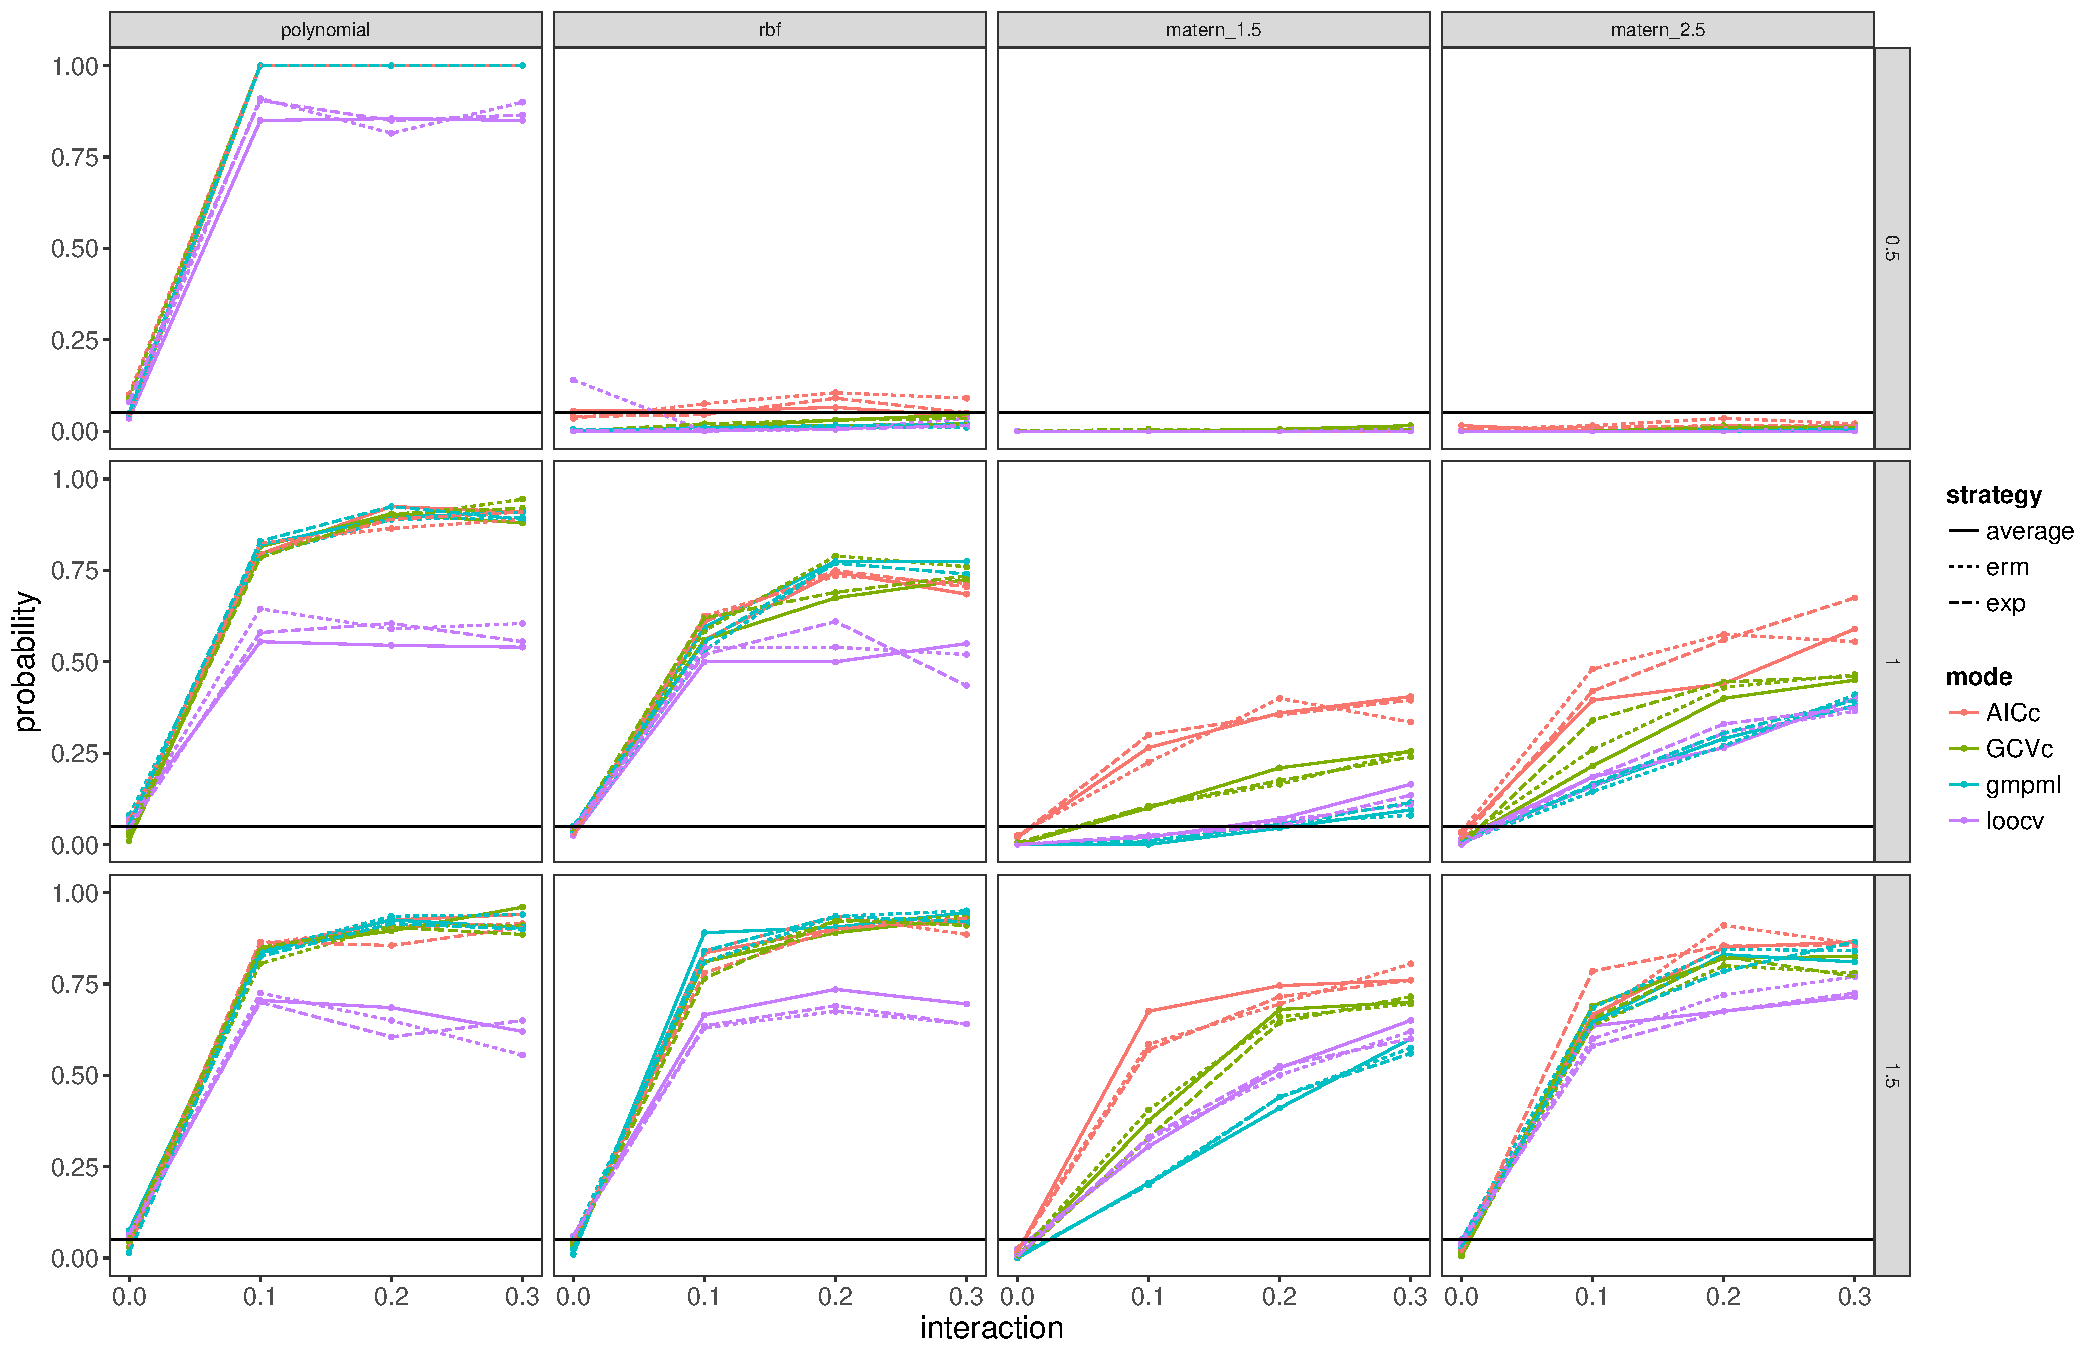
\includegraphics[width=0.9\columnwidth]{B1} 
\caption{Boot, True kernel only}
\label{fig:res}
\end{center}
\end{figure}

\begin{figure}
\begin{center}
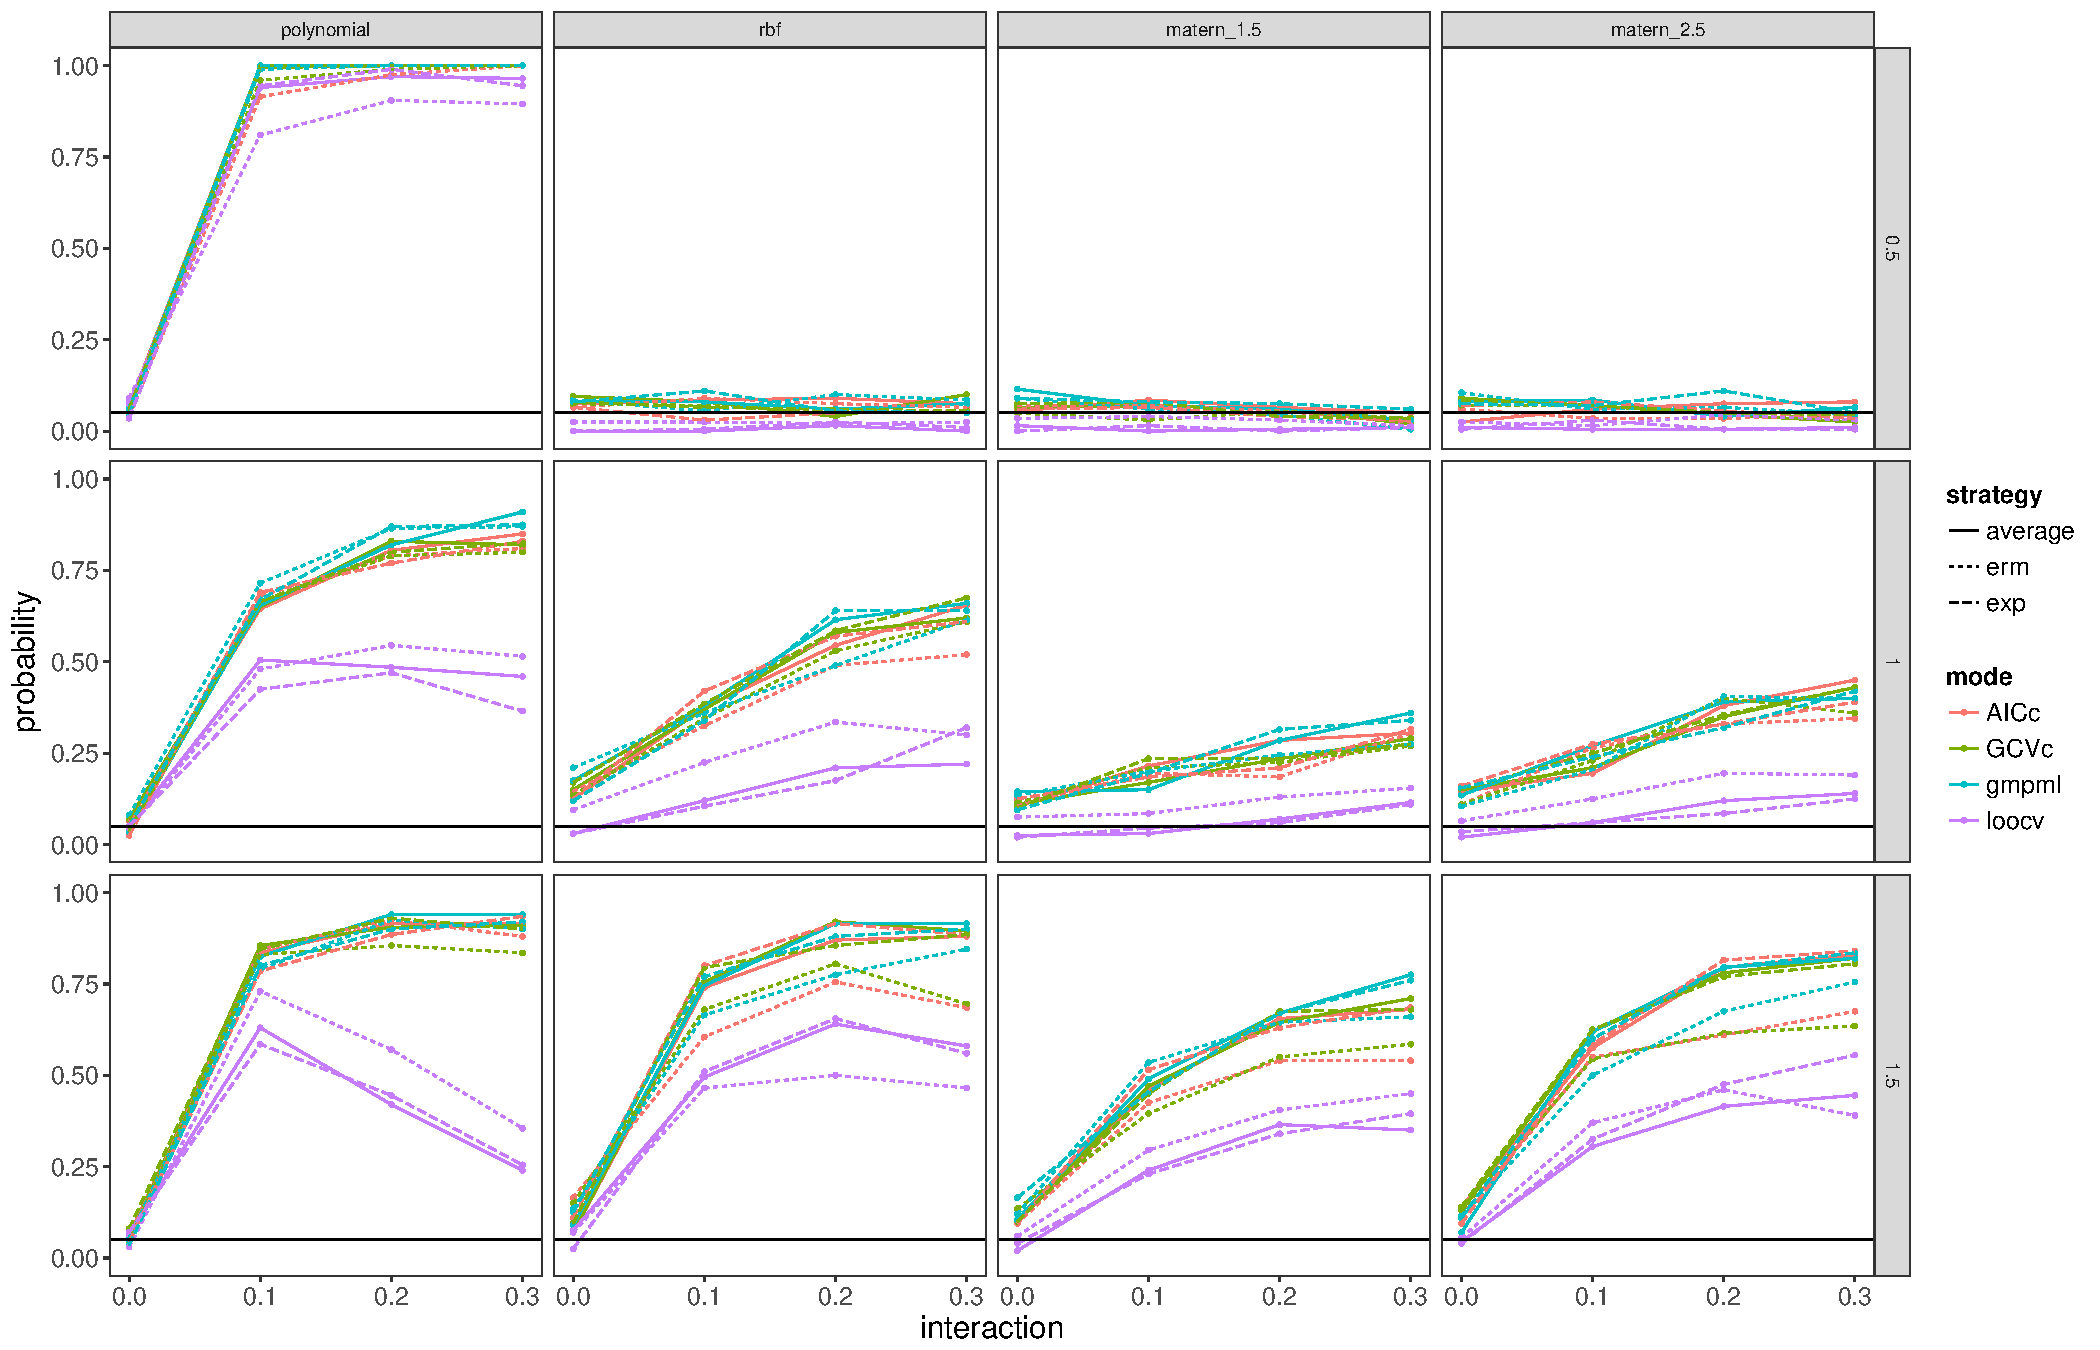
\includegraphics[width=0.9\columnwidth]{B2} 
\caption{Boot, 3 Polynomial kernels}
\label{fig:res}
\end{center}
\end{figure}

\begin{figure}
\begin{center}
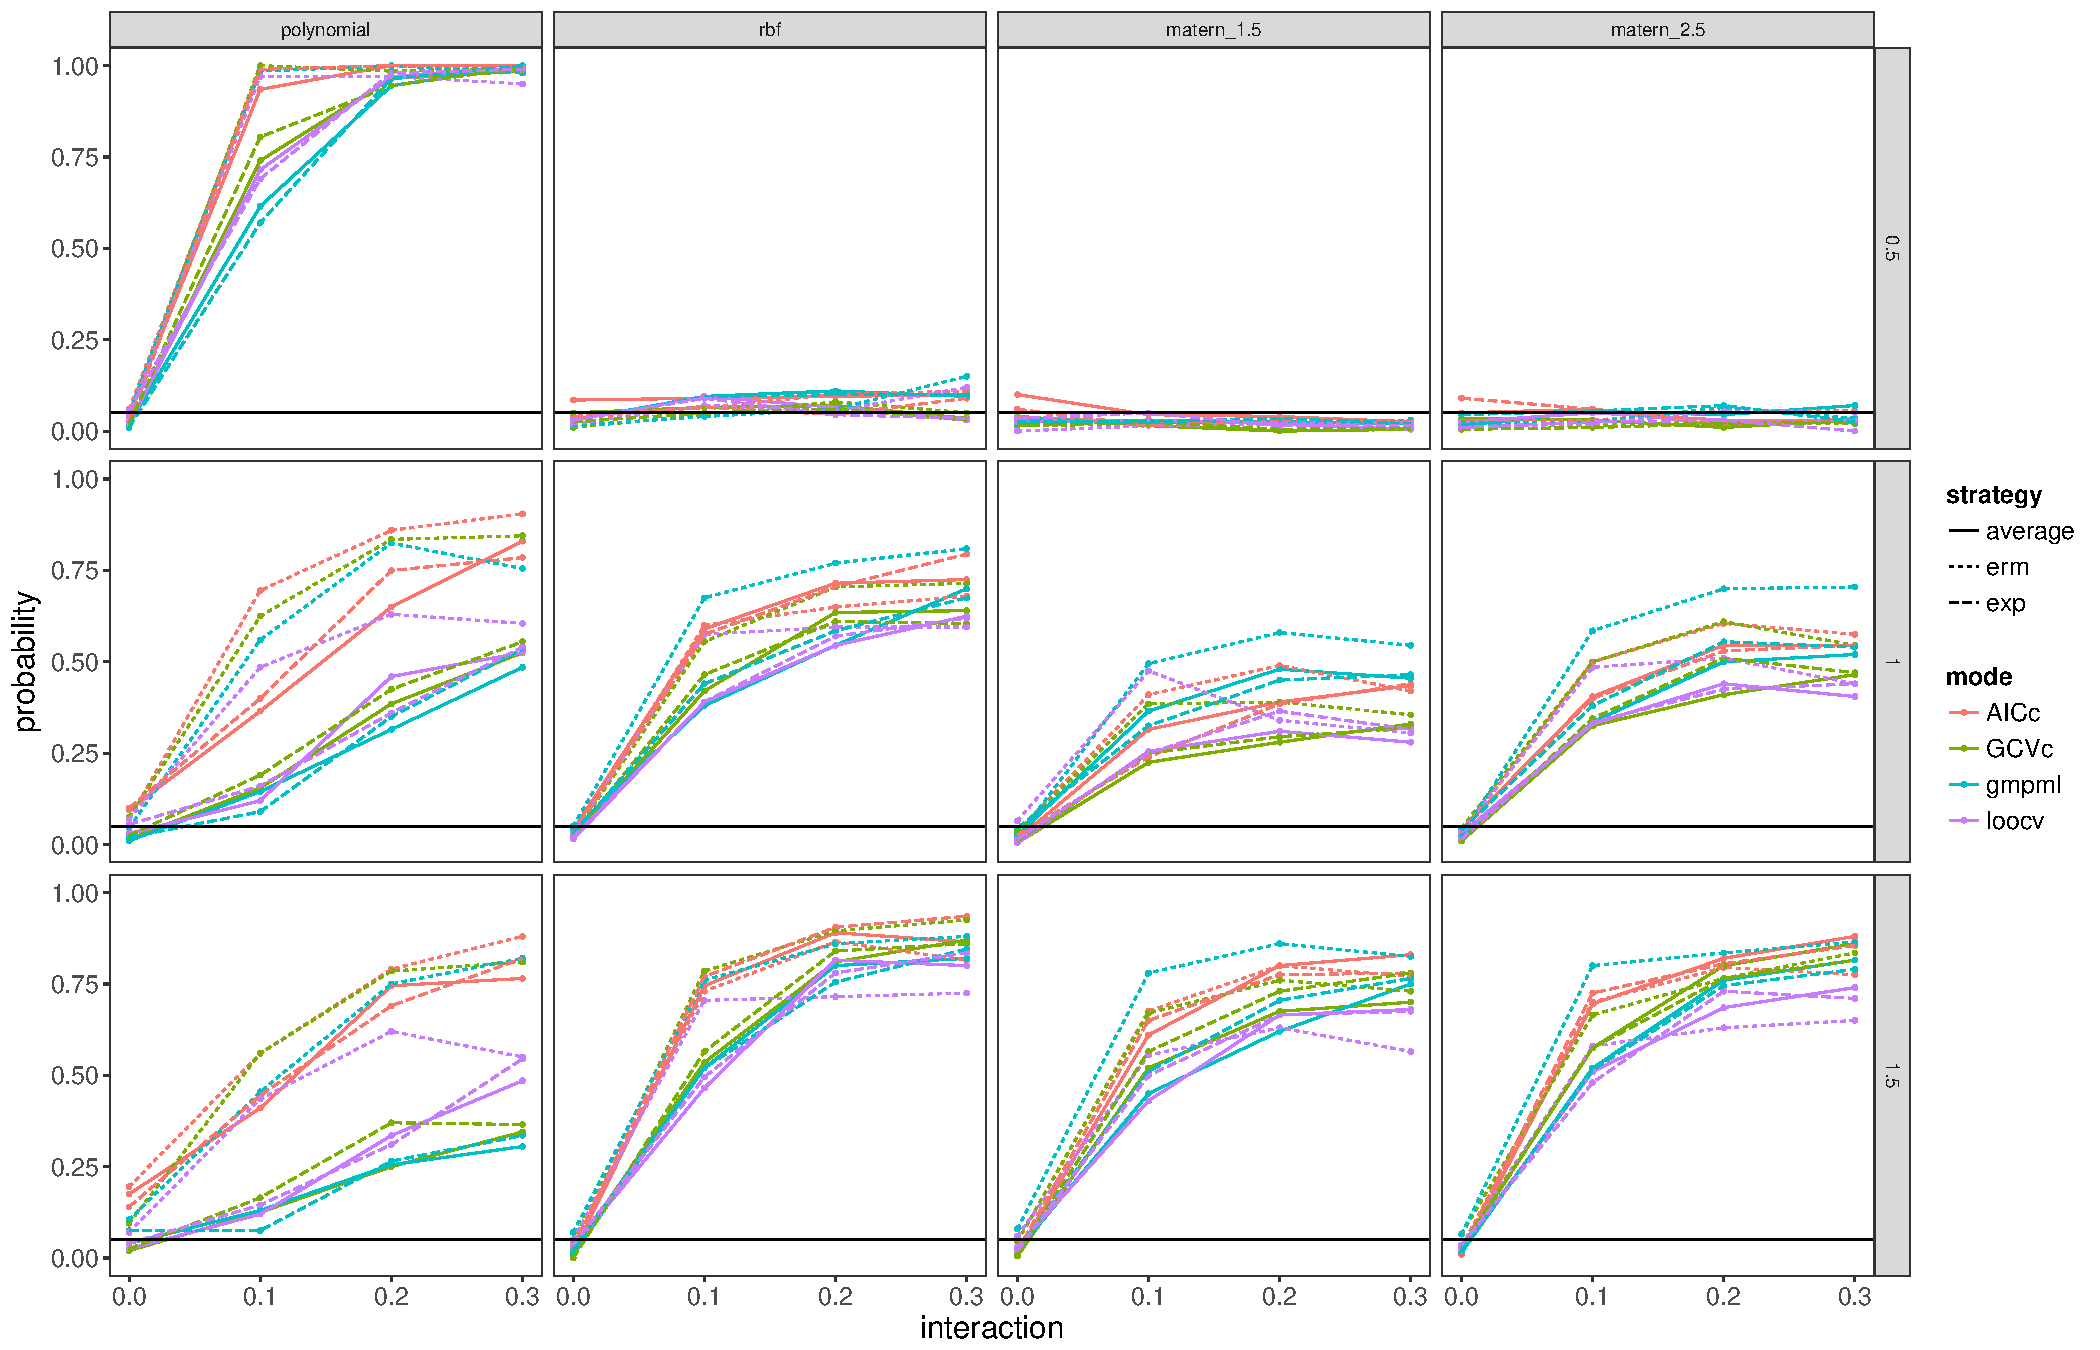
\includegraphics[width=0.9\columnwidth]{B3} 
\caption{Boot, 3 RBF kernels}
\label{fig:res}
\end{center}
\end{figure}

\begin{figure}
\begin{center}
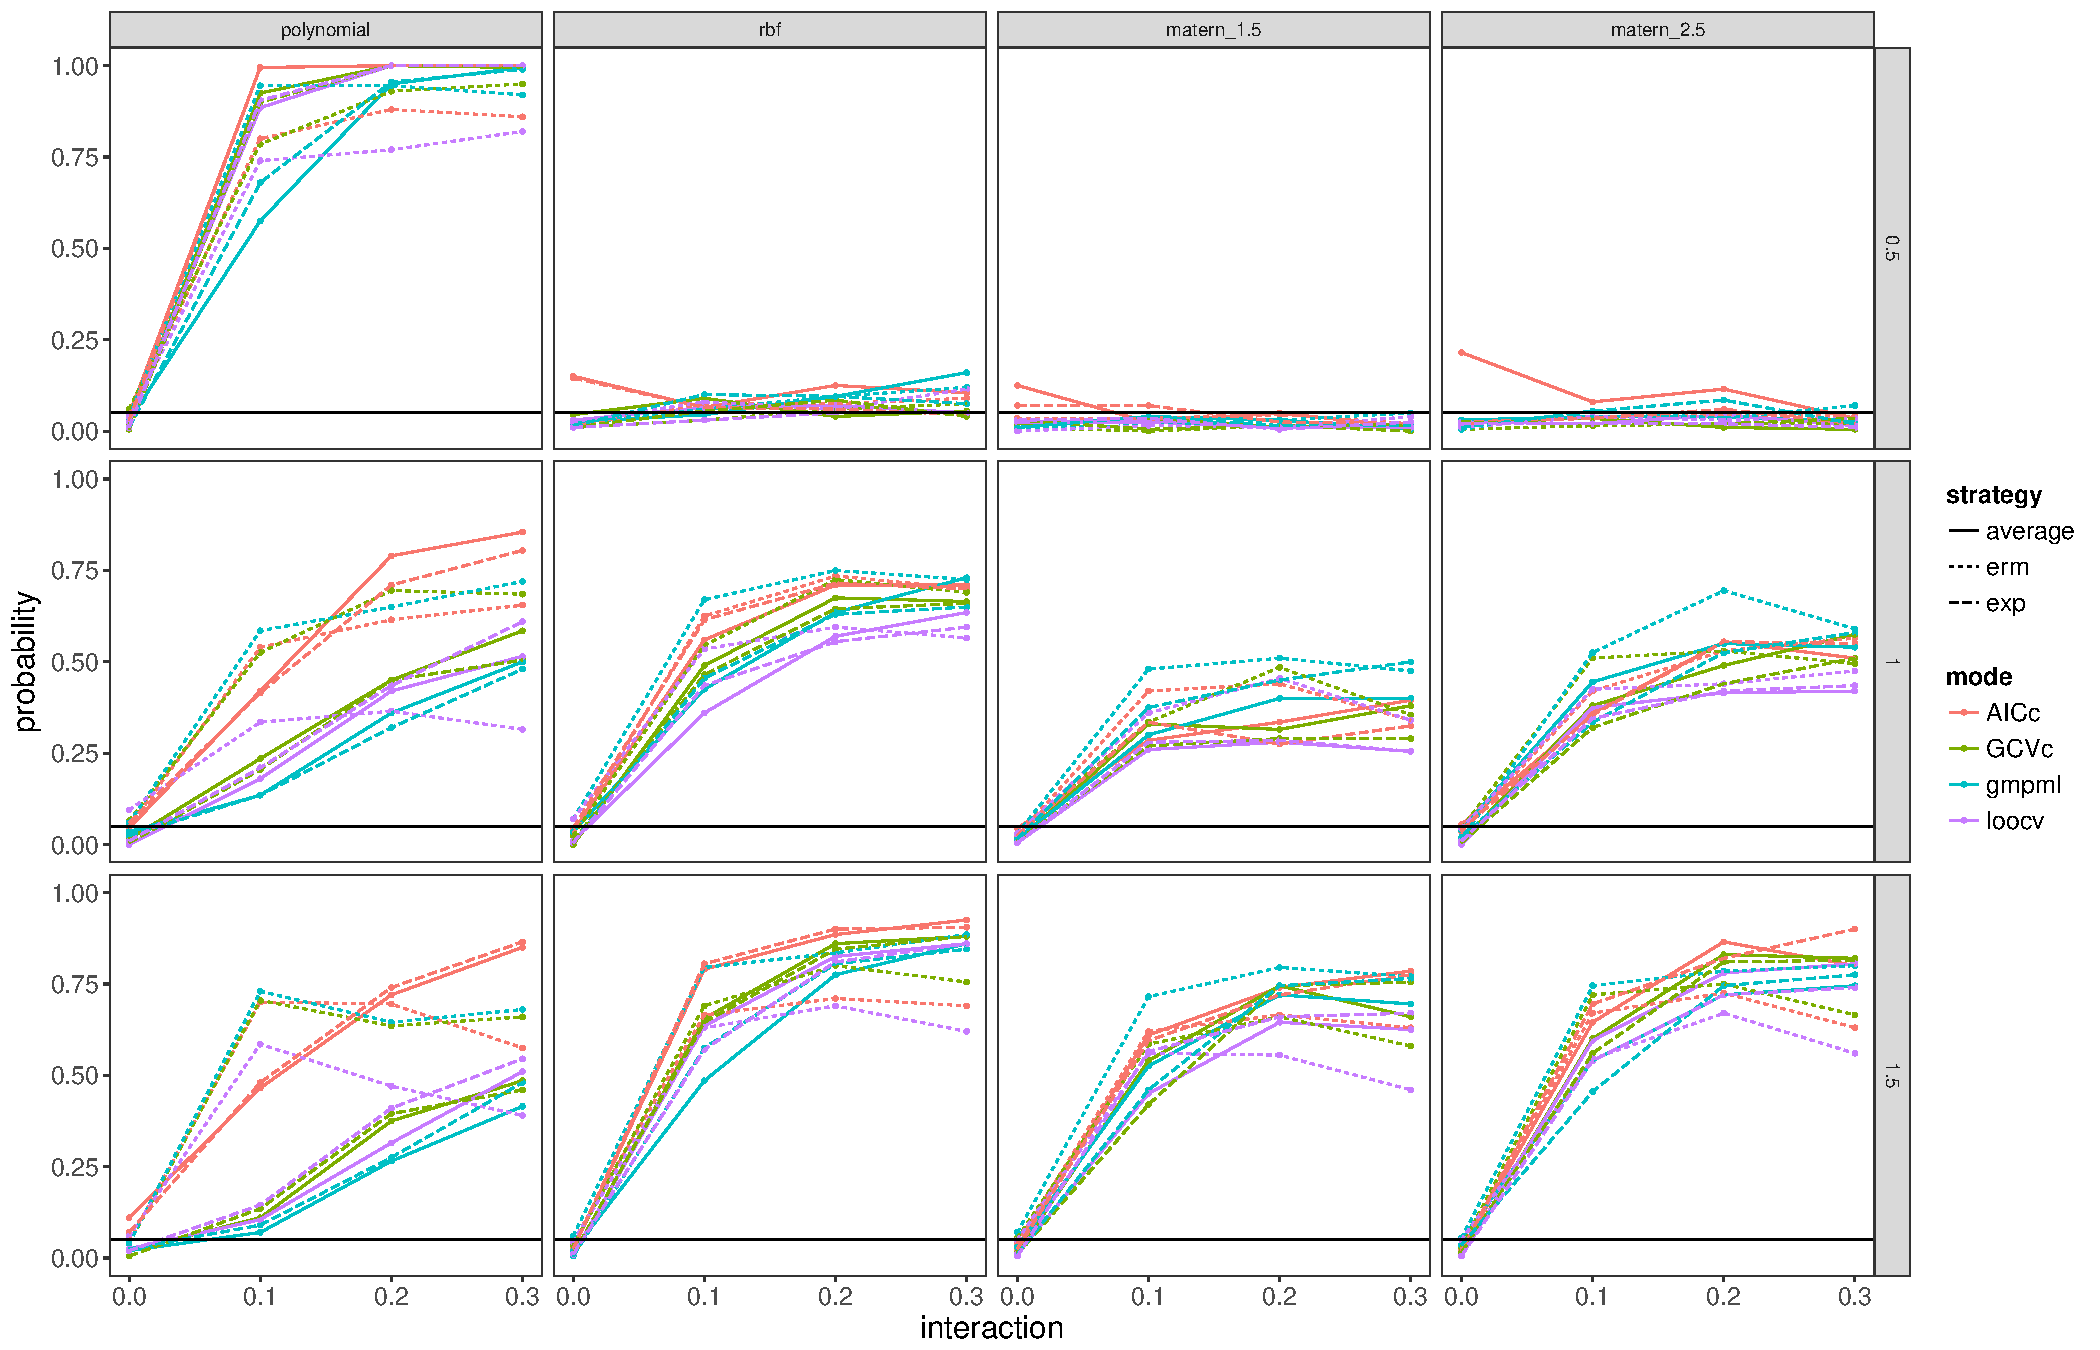
\includegraphics[width=0.9\columnwidth]{B4} 
\caption{Boot, 3 Polynomial kernels and 3 RBF kernels}
\label{fig:res}
\end{center}
\end{figure}

\begin{figure}
\begin{center}
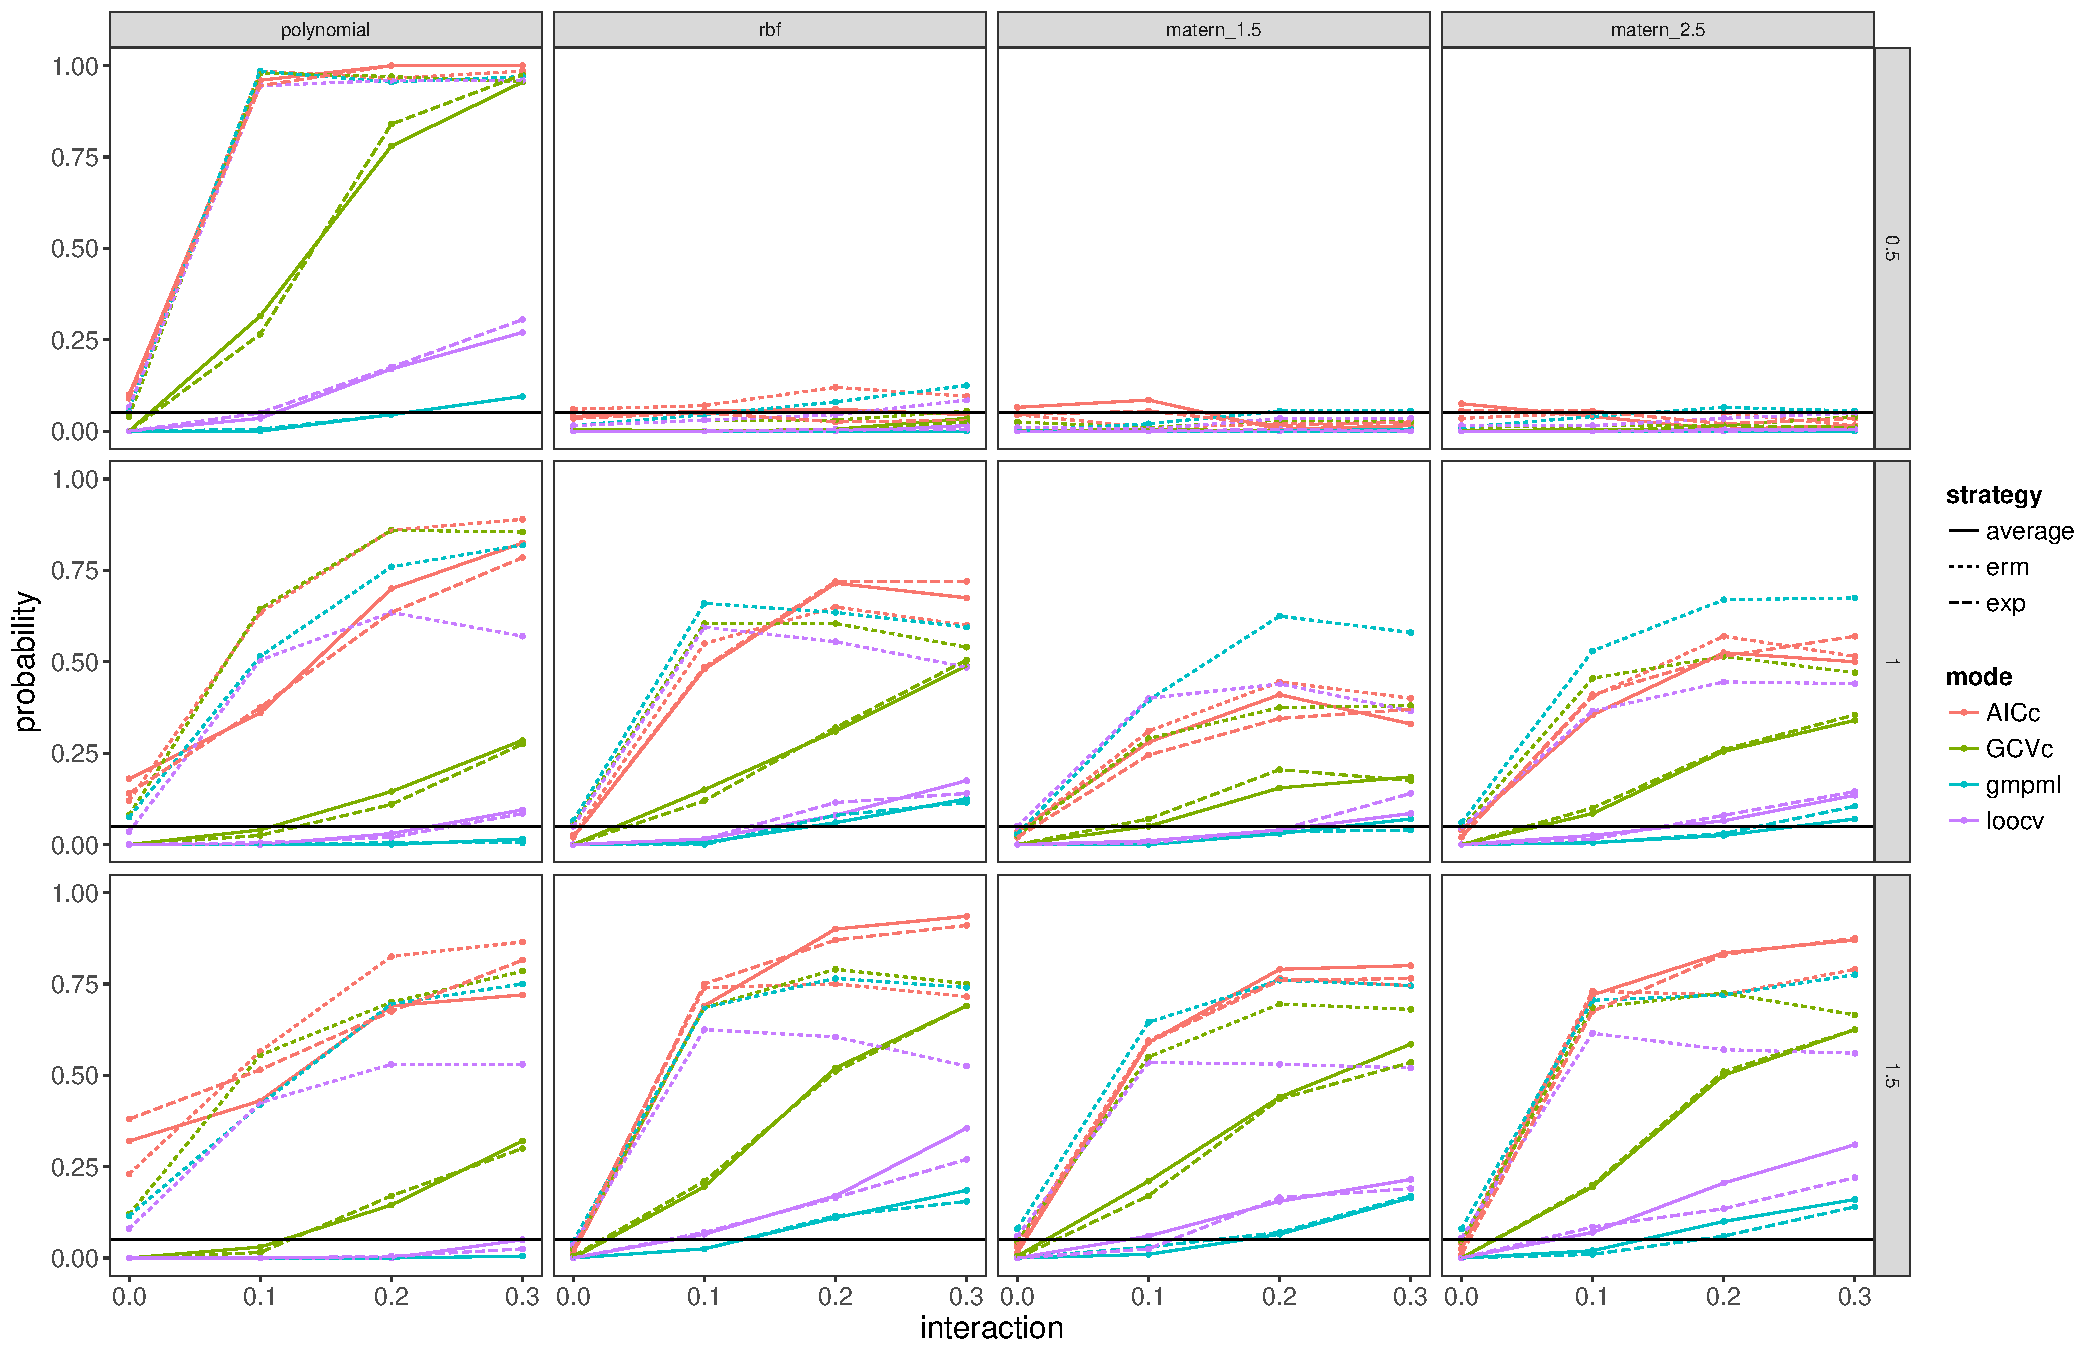
\includegraphics[width=0.9\columnwidth]{B5} 
\caption{Boot, 3 Matern kernels and 3 RBF kernels}
\label{fig:res}
\end{center}
\end{figure}

\begin{figure}
\begin{center}
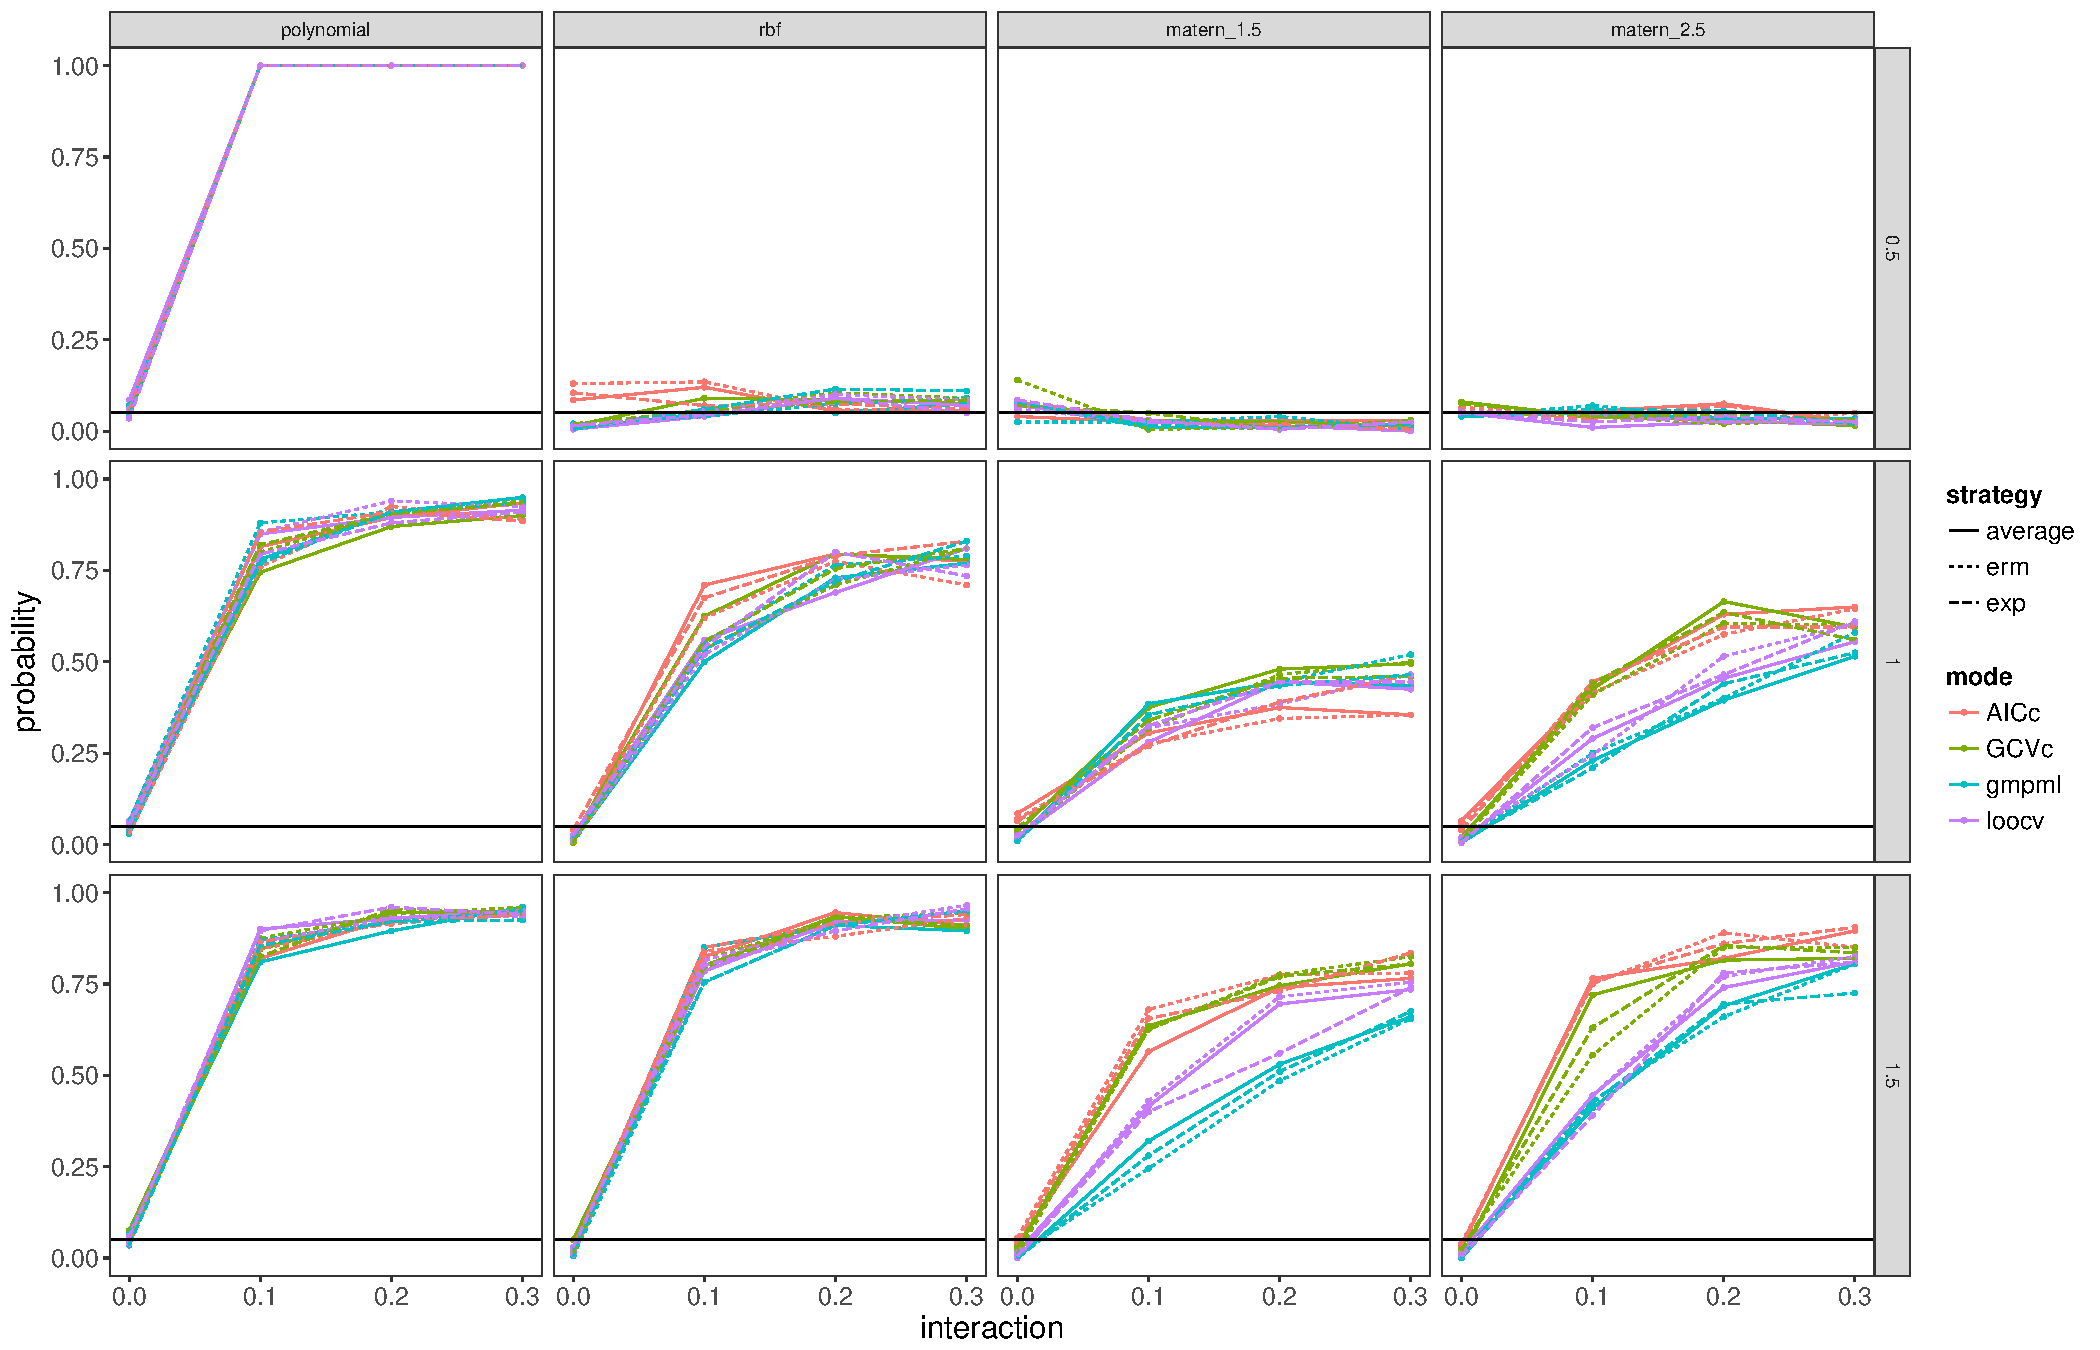
\includegraphics[width=0.9\columnwidth]{A1} 
\caption{Asym, True kernel only}
\label{fig:res}
\end{center}
\end{figure}

\begin{figure}
\begin{center}
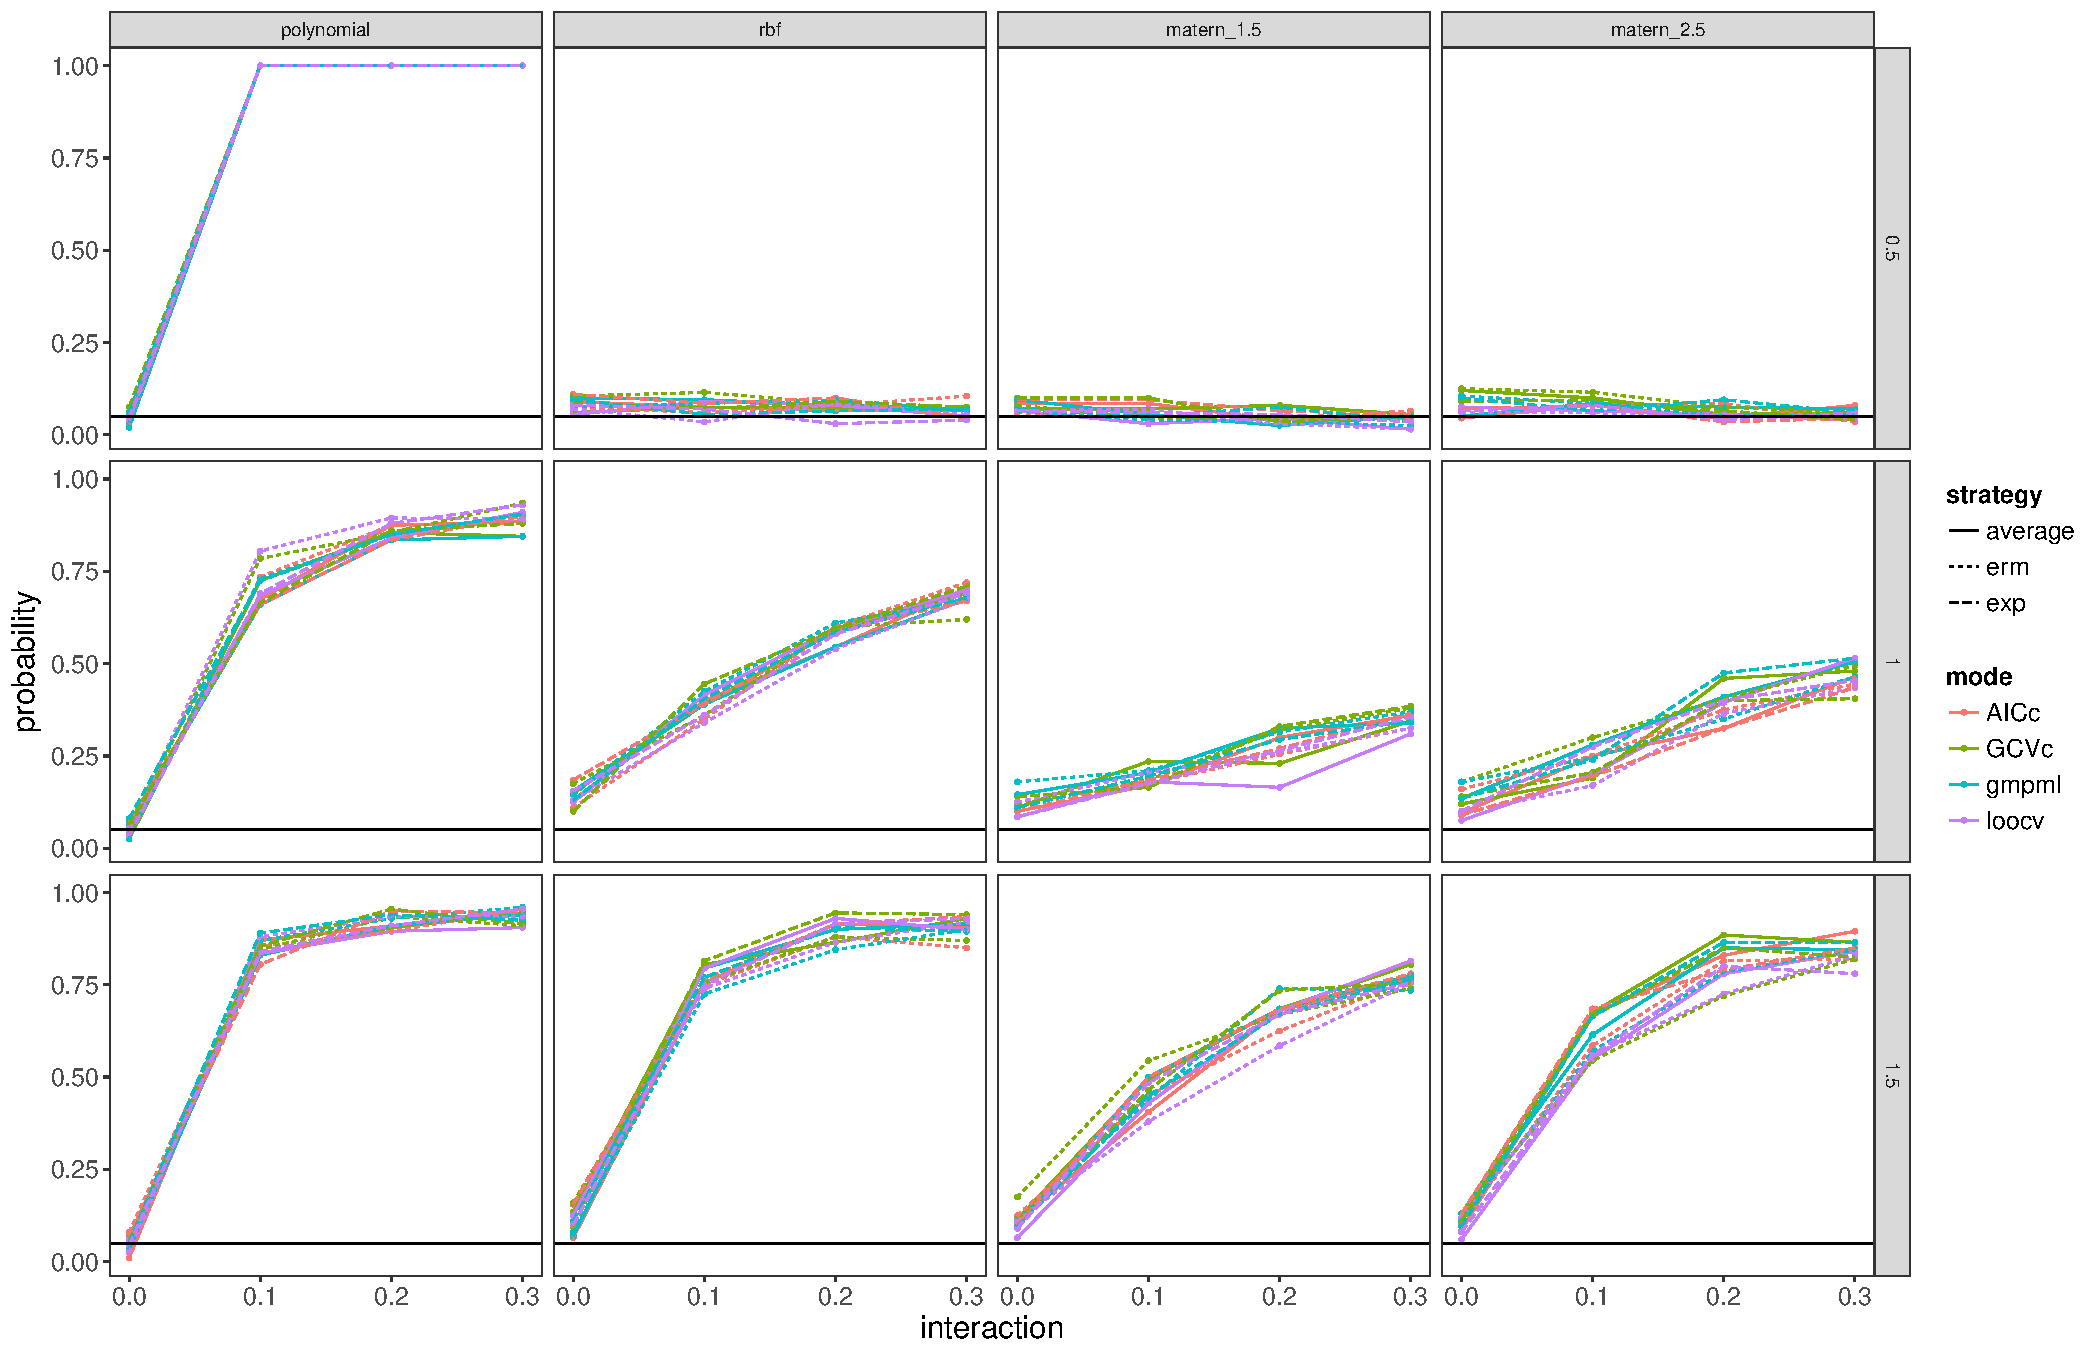
\includegraphics[width=0.9\columnwidth]{A2} 
\caption{Asym, 3 Polynomial kernels}
\label{fig:res}
\end{center}
\end{figure}

\begin{figure}
\begin{center}
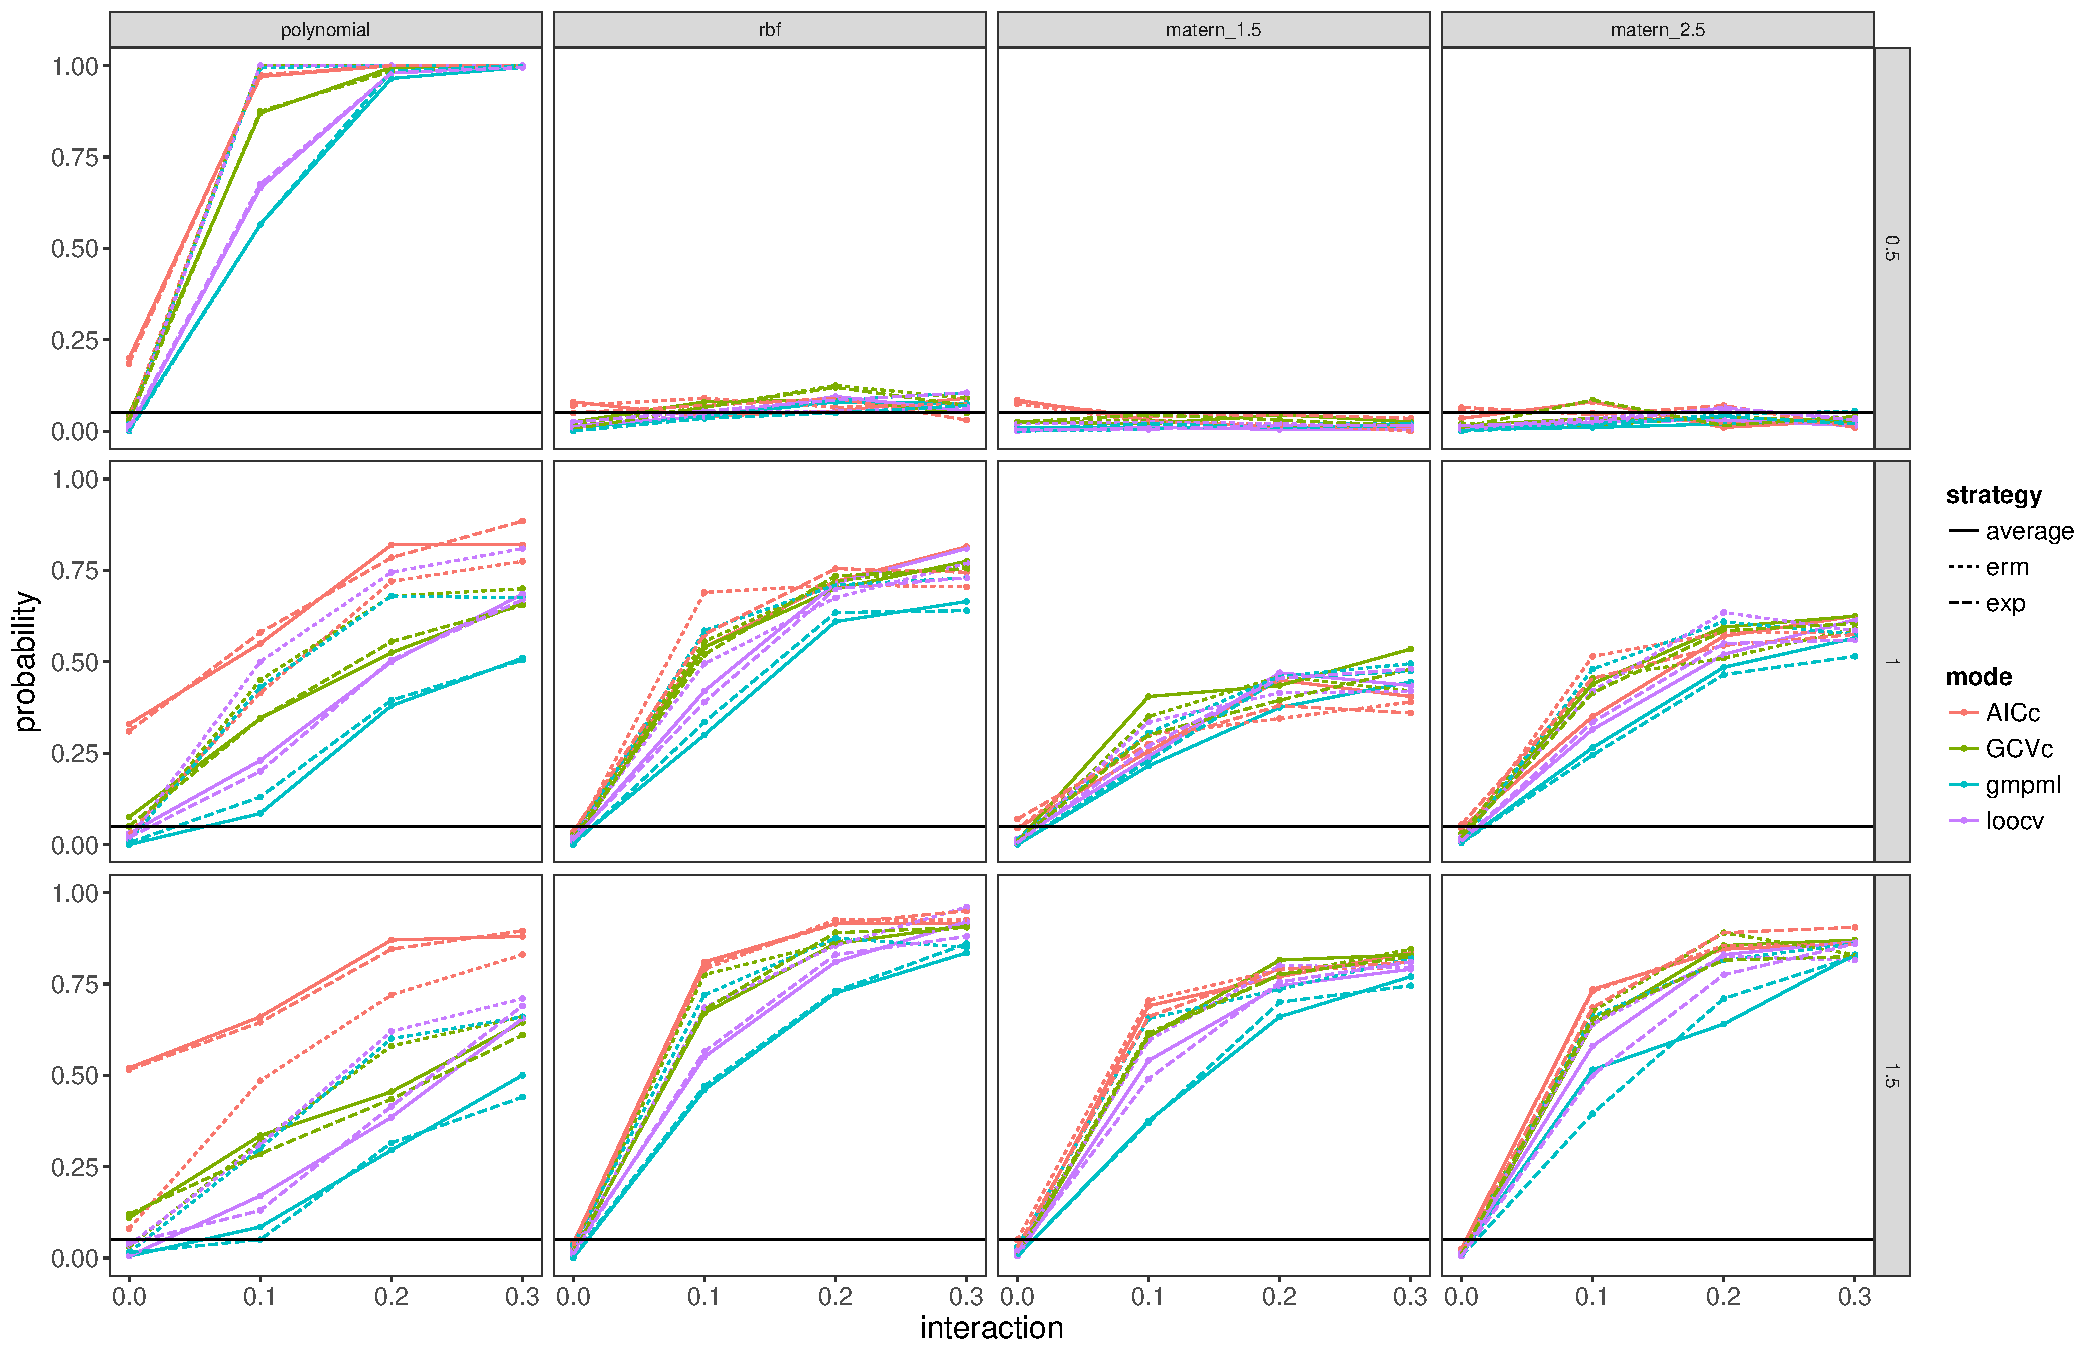
\includegraphics[width=0.9\columnwidth]{A3} 
\caption{Asym, 3 RBF kernels}
\label{fig:res}
\end{center}
\end{figure}

\begin{figure}
\begin{center}
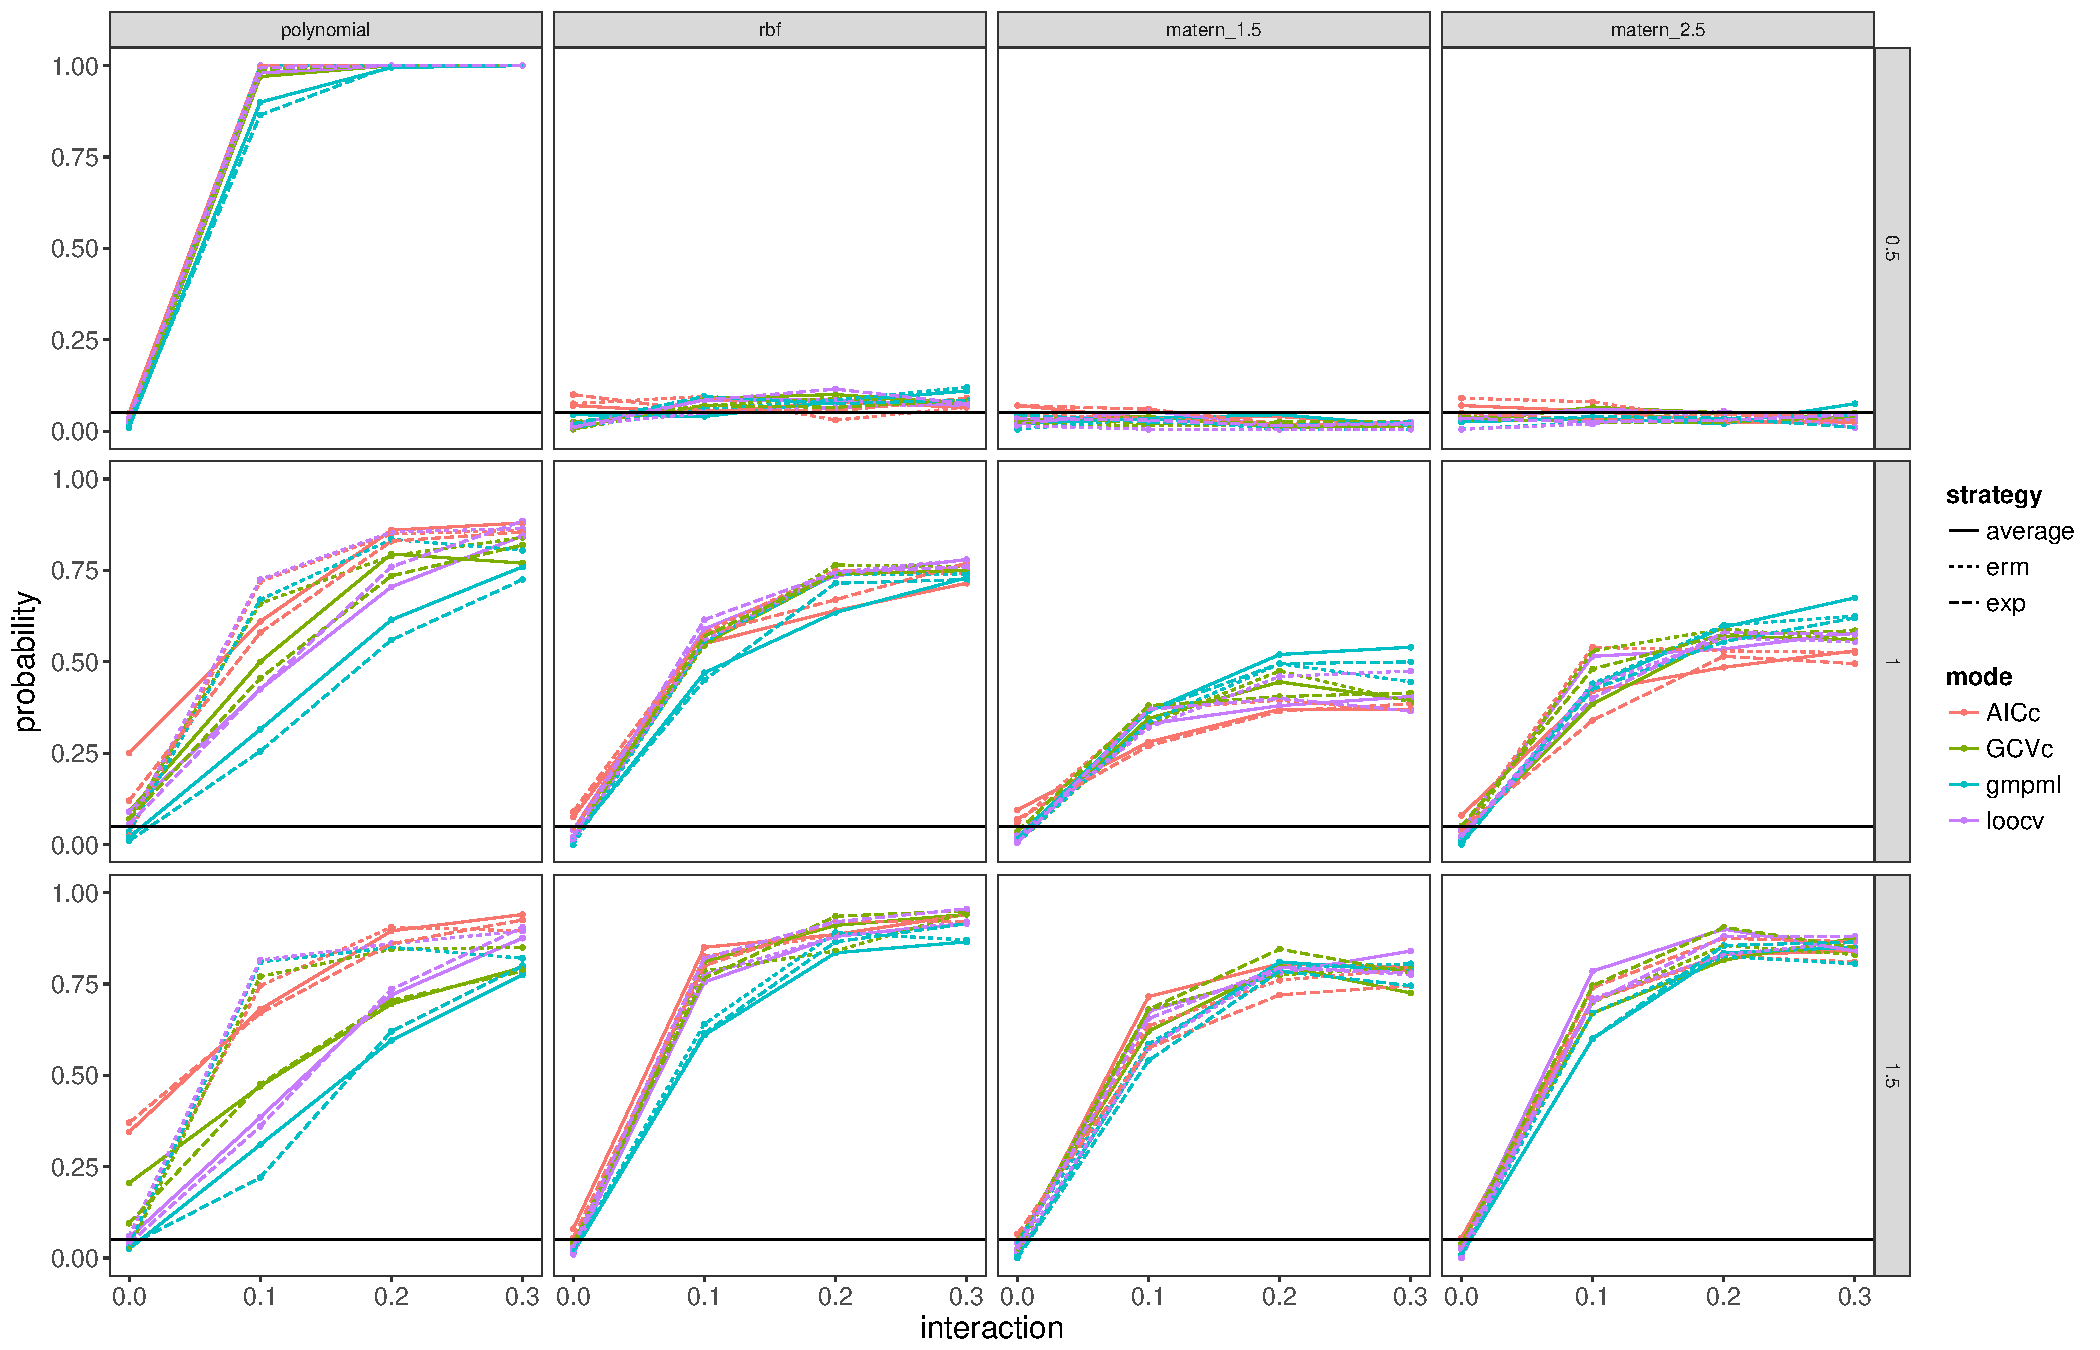
\includegraphics[width=0.9\columnwidth]{A4} 
\caption{Asym, 3 Polynomial kernels and 3 RBF kernels}
\label{fig:res}
\end{center}
\end{figure}

\begin{figure}
\begin{center}
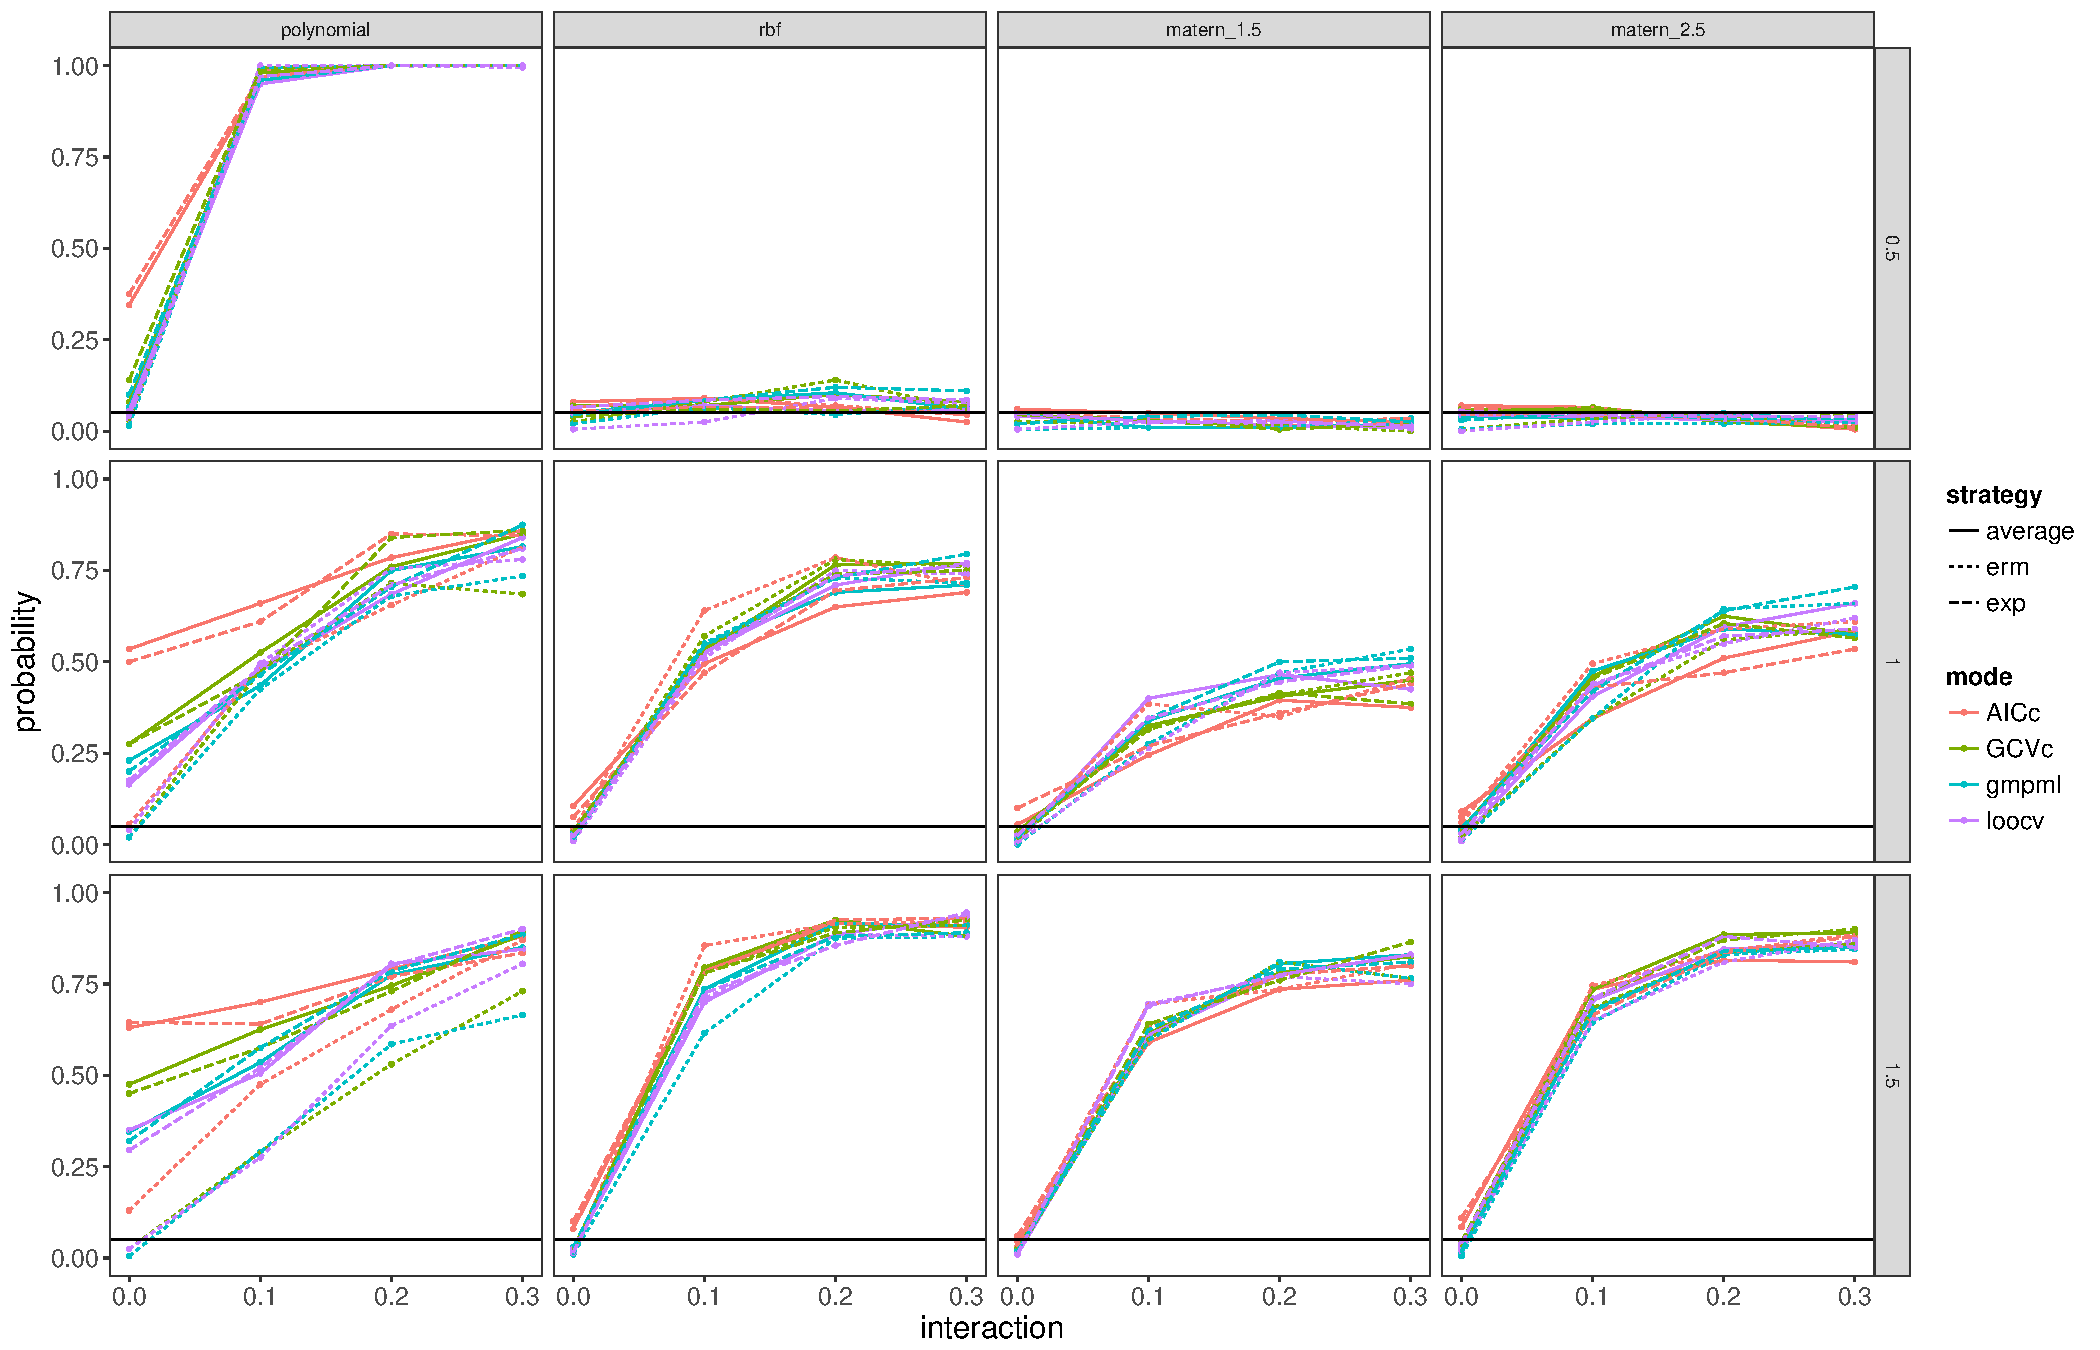
\includegraphics[width=0.9\columnwidth]{A5} 
\caption{Asym, 3 Matern kernels and 3 RBF kernels}
\label{fig:res}
\end{center}
\end{figure}

\begin{figure}
\begin{center}
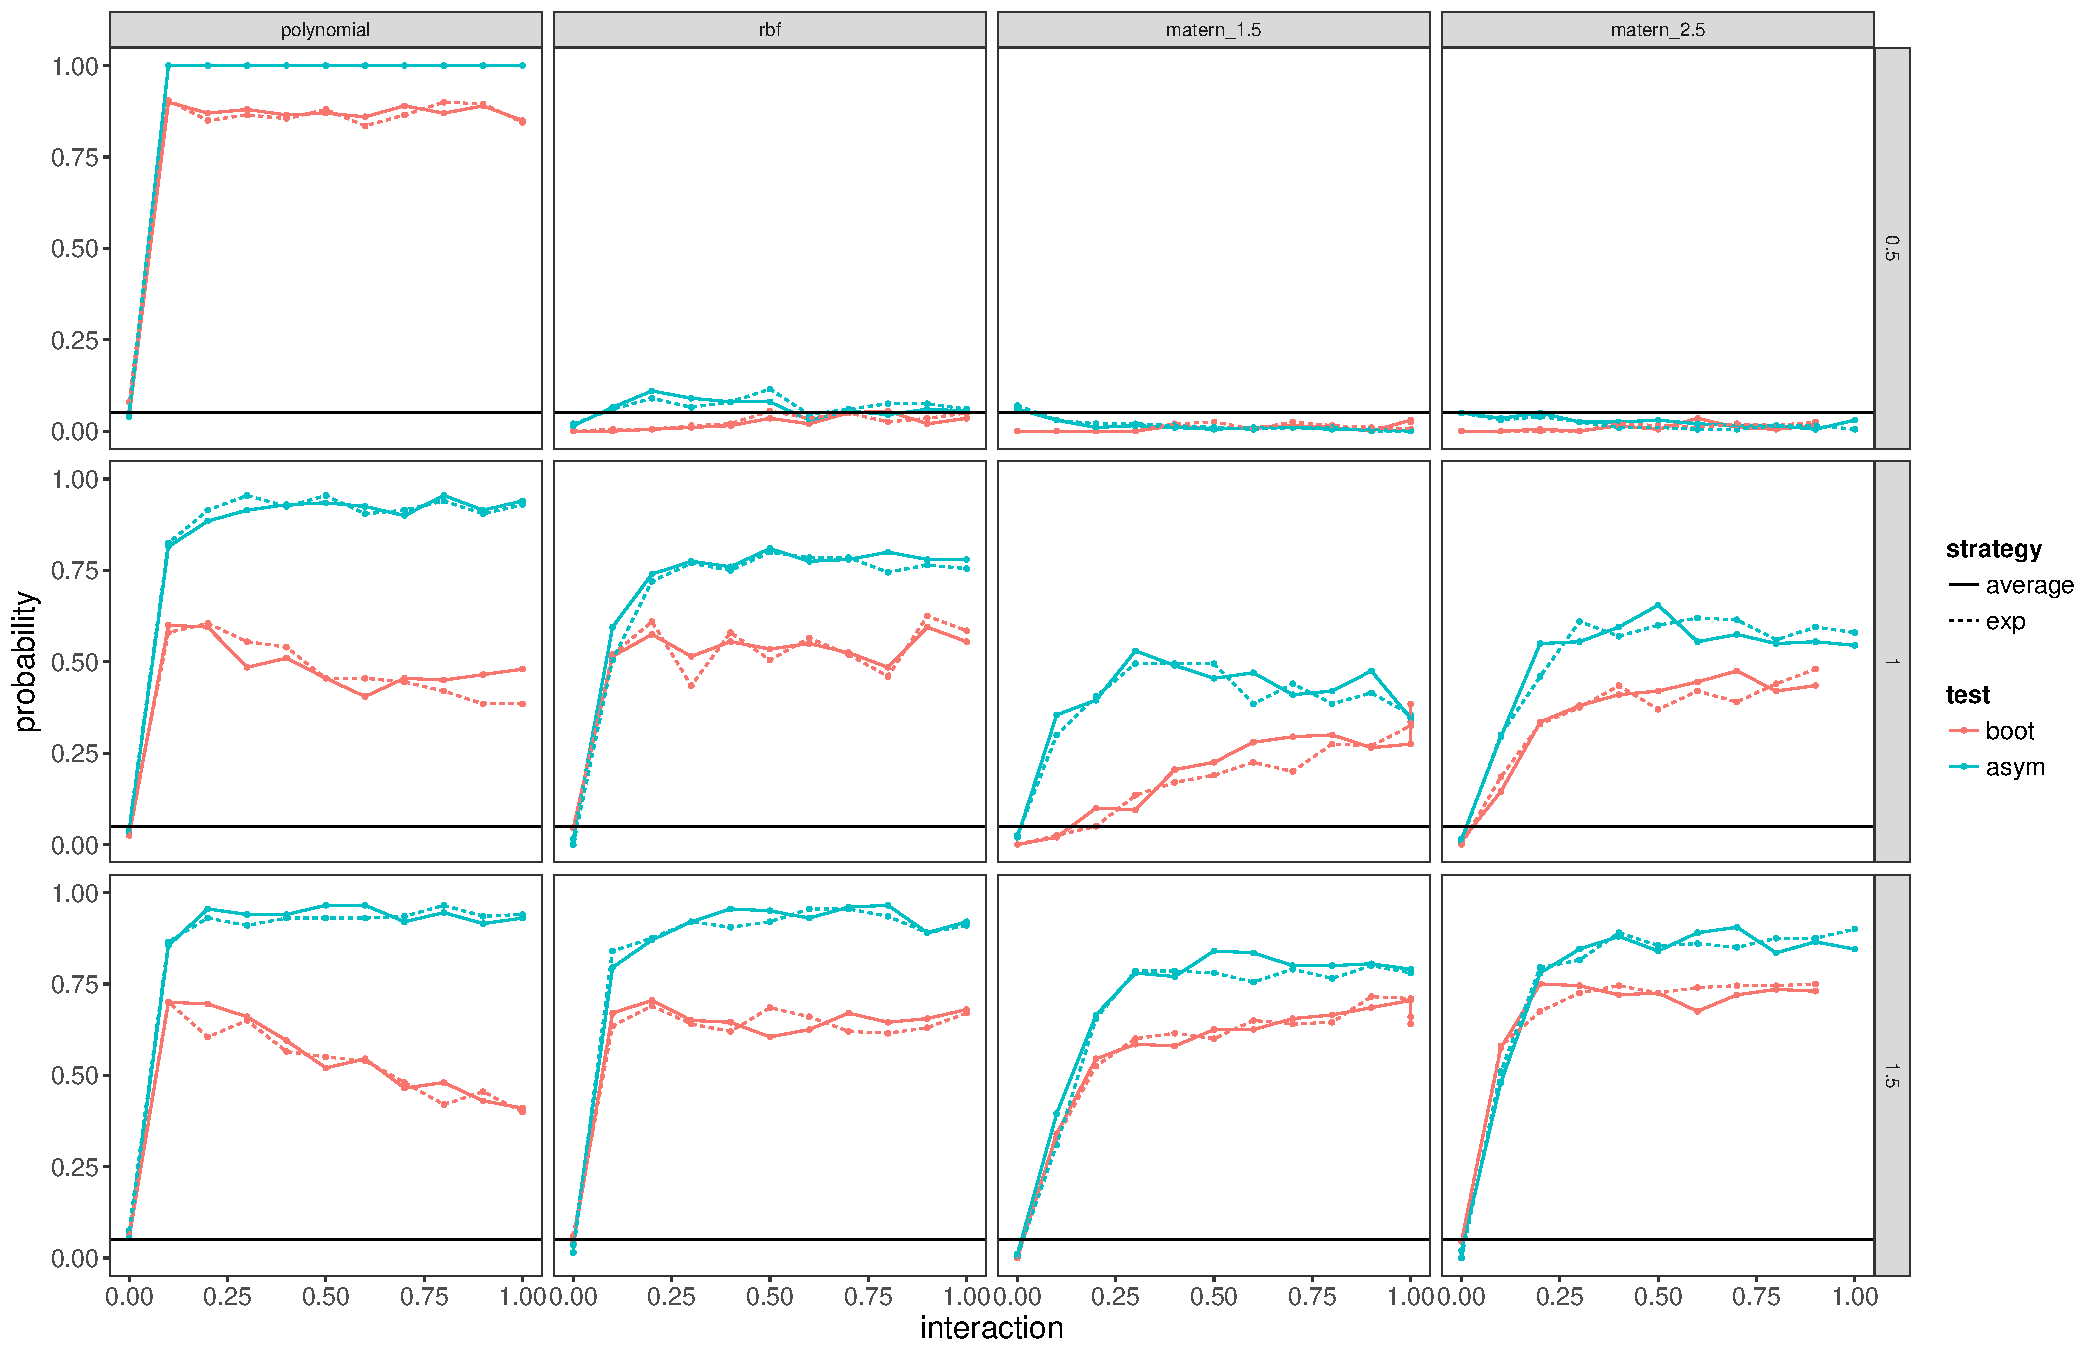
\includegraphics[width=0.9\columnwidth]{Both} 
\caption{Asym $\&$ Boot, True kernel only, n=100}
\label{fig:res}
\end{center}
\end{figure}

\begin{figure}
\begin{center}
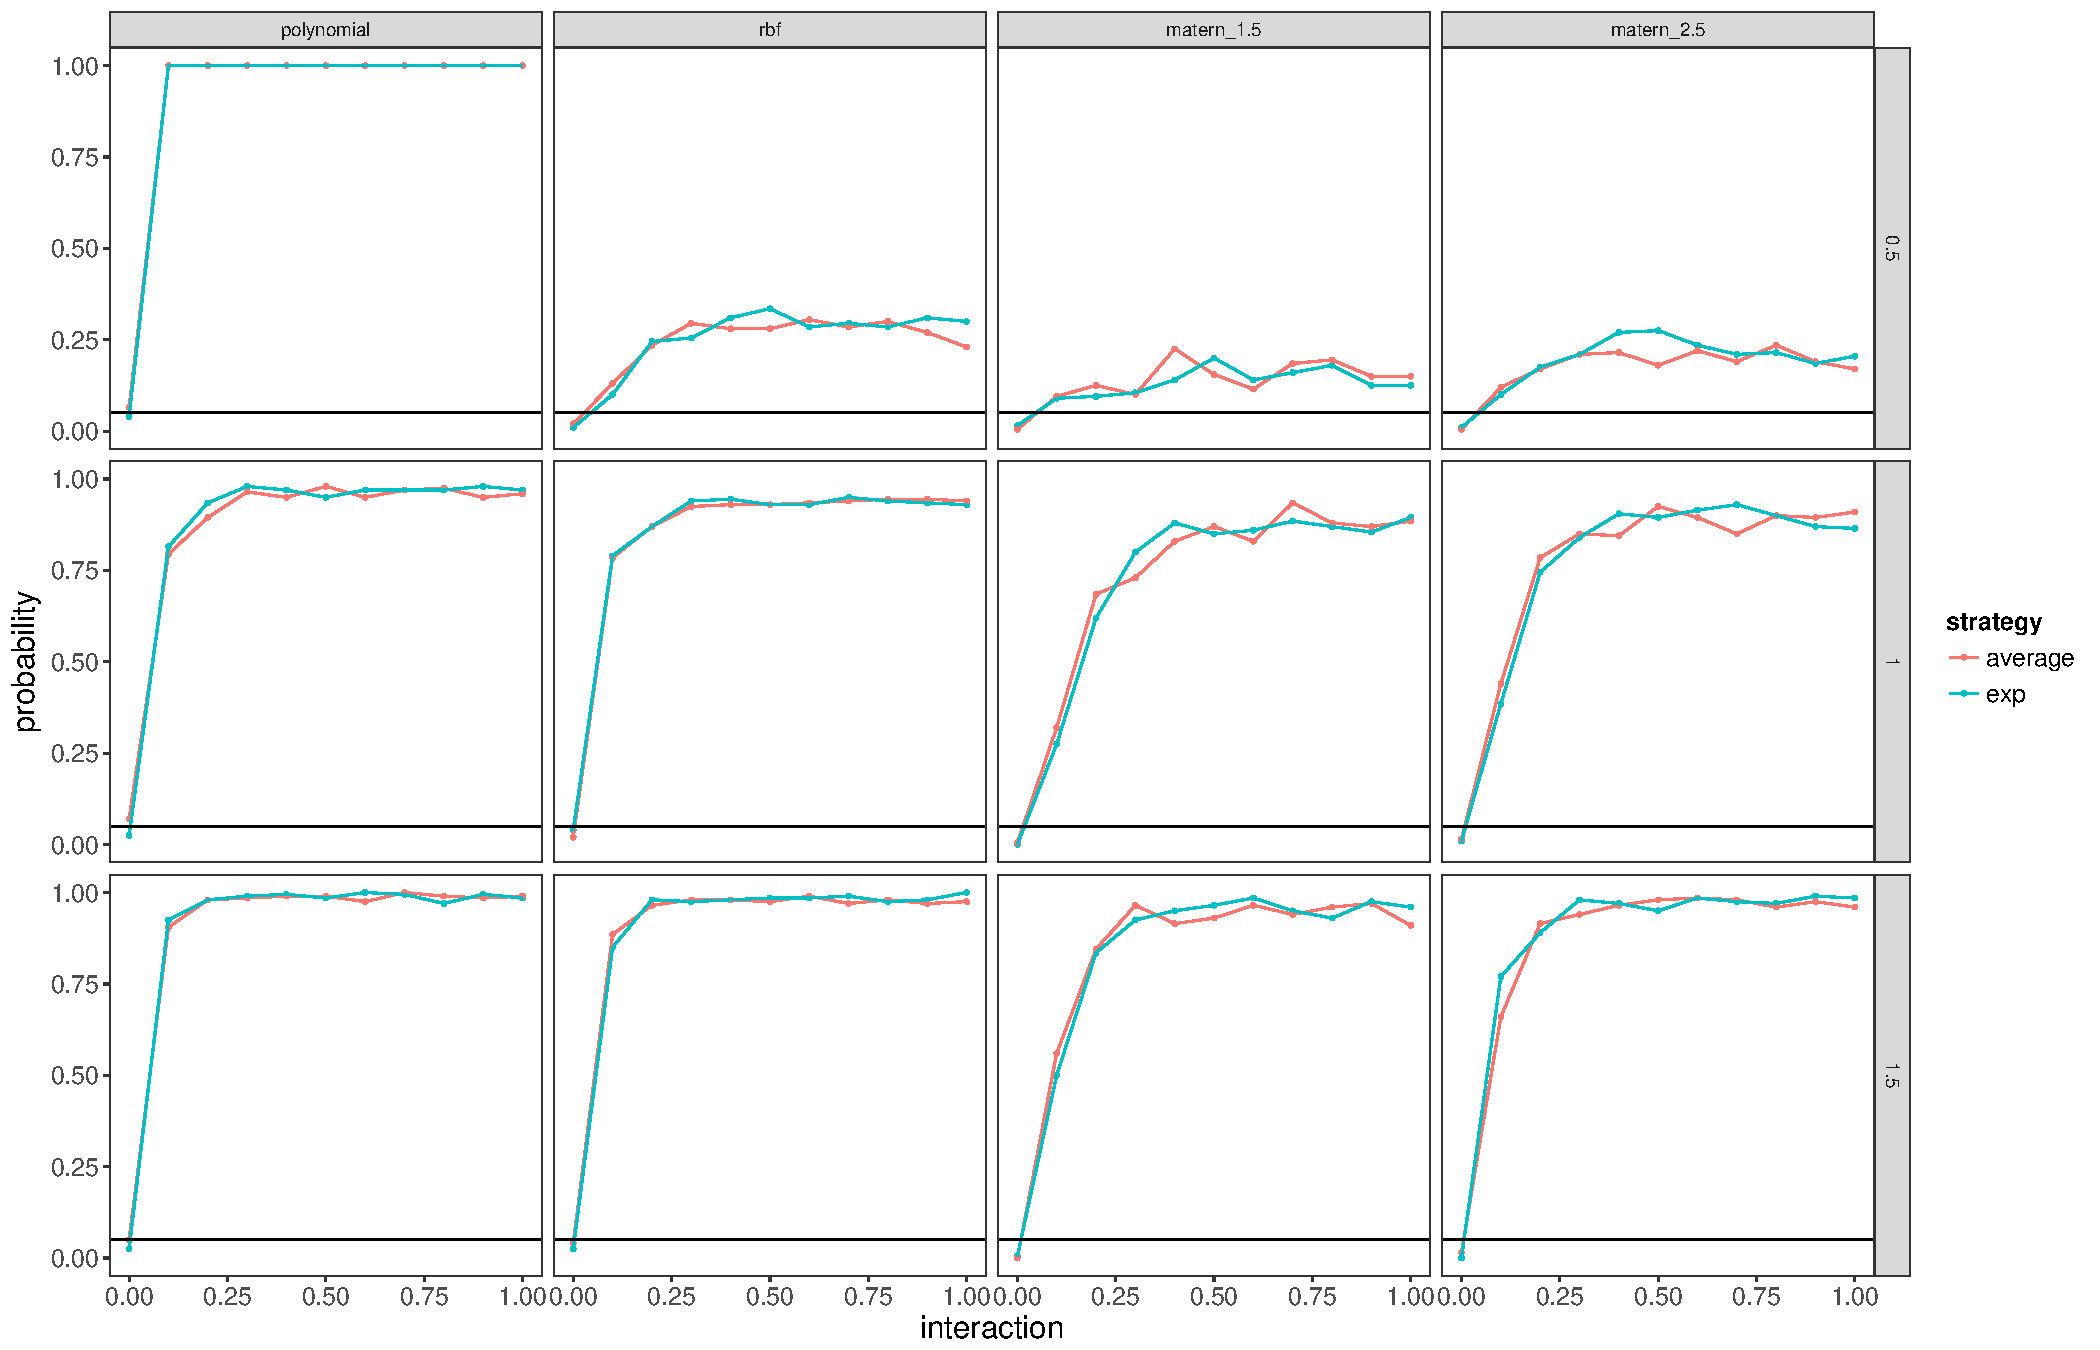
\includegraphics[width=0.9\columnwidth]{Asym_200} 
\caption{Asym, True kernel only, n=200}
\label{fig:res}
\end{center}
\end{figure}



\clearpage
\bibliography{reference}


%----------------------------------------------------------------------------------------
\end{document}
